\documentclass[twoside,notitlepage,11pt]{scrreprt}

\usepackage{graphicx}
\usepackage{amsfonts}
\usepackage{amsbsy}
\usepackage{verbatimfile}
\usepackage{fancyhdr}
% The next rawfonts package one is used in the ``datablad''.
%FIXME\usepackage[only,egtrm]{rawfonts}
% Handle sorting in reference list
%FIXME package is obsolete \usepackage{citesort}
% Create an index table
\usepackage{makeidx}
% For html links in install chapter (install latex2html package to get
% this style)
\usepackage{html}
\usepackage{color}
\usepackage{xcolor}
\usepackage{listings}
\usepackage{xspace}
\usepackage{mhchem}

\definecolor{srcback}{rgb}{1,0.8,0.1}

\lstset{ %
language=C++,                % choose the language of the code
basicstyle=\footnotesize,       % the size of the fonts that are used for the code
numbers=left,                   % where to put the line-numbers
numberstyle=\footnotesize,      % the size of the fonts that are used for the line-numbers
stepnumber=1,                   % the step between two line-numbers. If it is 1 each line will be numbered
numbersep=5pt,                  % how far the line-numbers are from the code
backgroundcolor=\color{srcback},  % choose the background color. You must add \usepackage{color}
showspaces=false,               % show spaces adding particular underscores
showstringspaces=false,         % underline spaces within strings
showtabs=false,                 % show tabs within strings adding particular underscores
frame=single,           % adds a frame around the code
tabsize=2,          % sets default tabsize to 2 spaces
captionpos=b,           % sets the caption-position to bottom
breaklines=true,        % sets automatic line breaking
breakatwhitespace=false,    % sets if automatic breaks should only happen at whitespace
escapeinside={\%*}{*)}          % if you want to add a comment within your code
}

\newcommand{\smallverbatimfile}[1]{{\footnotesize\verbatimfile{#1}}}

\def\reportnum{Ris{\o}--R--1416(rev.ed.)(EN)}



\newcommand{\MCS}{McStas\xspace}
\newcommand{\version}{{2.0}}
\newcommand{\reldate}{{Sep, 2013}}
\newcommand{\Ombold}{\mbox{\boldmath $\Omega$}}



% enable index generation
\makeindex


\begin{document}

%\maketitle
%FIXME \input{risoe-rep-title}

\thispagestyle{empty}
% Emacs settings: -*-mode: latex; TeX-master: "manual.tex"; -*-

\begin{abstract}
\input{abstract}
\end{abstract}

\vskip\baselineskip\noindent
This report documents \MCS\ version \version, released \reldate
\vskip\baselineskip\noindent
The authors are:
\begin{quote}
\label{p:authors}
Peter Kj\ae r Willendrup \verb+<peter.willendrup@risoe.dk>+ \\
Materials Research Department, Ris{\o} National Laboratory, DTU, Roskilde, Denmark 

Emmanuel Farhi \verb+<farhi@ill.fr>+ \\
Institut Laue-Langevin, Grenoble, France 

Kim Lefmann \verb+<kim.lefmann@risoe.dk>+ \\
Materials Research Department, Ris{\o} National Laboratory, DTU, Roskilde, Denmark 

\end{quote}
as well as authors who left the project:
\begin{quote}
Peter Christiansen \verb+<pchristi@hep.lu.se>+\\
Materials Research Department, Ris{\o} National Laboratory, Roskilde, Denmark\\
Present address: University of Lund, Lund, Sweden\\
Klaus Lieutenant \verb+<Klaus.Lieutenant@ife.no>+ \\
Institut Laue-Langevin, Grenoble, France \\
Present address: Institute for Energy Technology, Kjeller, Norway \\
Kristian Nielsen \verb+<kristian-nielsen@mail.tele.dk>+ \\
Materials Research Department, Ris{\o} National Laboratory, Roskilde, Denmark\\
Presently associated with: MySQL AB, Sweden
\end{quote}
%Front page illustration:\\[\baselineskip]
%Simulated scattering from a vanadium sample
%taking into account the secondary extinction. See
%section~\ref{s:vanadium-result}.
\vfill
\noindent ISBN 978--87--550--3617--8
\par\noindent ISSN 0106--2840
\par\noindent\hbox{}\hfill
    Pitney Bowes Management Services Denmark A/S $\cdot$ Ris{\o} National Laboratory $\cdot$ \number\year
%    Information Service Department $\cdot$ Ris{\o} $\cdot$ \number\year
\par
\thispagestyle{empty}\clearpage





\tableofcontents

%FIXME % Emacs settings: -*-mode: latex; TeX-master: "manual.tex"; -*-

\addcontentsline{toc}{chapter}{\protect\numberline{}{Preface and acknowledgements}}
\chapter*{Preface and acknowledgements}
This document contains information on the Monte Carlo neutron
ray-tracing program \MCS\ version \version, an update to the initial
release in October 1998 of version 1.0 as presented in Ref.~\cite{nn_10_20}. The reader of this
document is supposed to have some knowledge of neutron scattering,
whereas only little knowledge about simulation techniques is
required. In a few places, we also assume familiarity with the
use of C, UNIX and of the world wide web (WWW).

It is a pleasure to thank Prof.~Kurt N.~Clausen for his continuous
support to this project and for having initiated the work in the first
place. 
%Both he and our other collaborators, Henrik M.\ R\o nnow and Mark
%Hagen have made major contributions to the project.  Also the
%contributions from our test users, the students Asger Abrahamsen, Niels
%Bech Christensen, and Erik Lauridsen, are gratefully acknowledged; they
%gave us an excellent opportunity to pinpoint a vast amount of serious
%errors in the test version.  Useful comments to this document itself
%have been given by Bella Lake and Alan Tennant.  
We have also benefited
from discussions with many other people in the neutron scattering
community, too numerous to mention here.

%Philipp Bernhardt contributed the two chopper components in
%sections~\ref{s:chopper} and~\ref{s:first_chopper}. Emmanuel Farhi
%contributed the components in sections~\ref{s:sourceoptimizer},
%\ref{s:monitornd}, and~\ref{s:monitoroptimizer}. We encourage other
%users to contribute components with manual entries for inclusion in
%future versions of \MCS.

This project has been supported by the European Union
through the XENNI program and the RTD ``Cool Neutrons'' and ``SCANS'' programs.

In case of any errors, questions, suggestions, %or other need for support should arise,
%do not hesitate to 
contact the authors at \verb+mcstas@risoe.dk+
or consult the \MCS\ WWW home page~\cite{mcstas_webpage}.

New features in \MCS\ version \version\ as compared to version 1.4 include

\begin{itemize}
\item A three-component representaton, (s$_x$, s$_y$, s$_z$), of the neutron spin has been added, 
which includes the possibility for simulations of polarisation instruments.
\item A signal handling system has been added, which gives the possibility for interacting with a
running simulation
\item The list of available kernel calls have been extended. They are normally used by users coding
new components. The new kernel calls include the name, position and orientation of components.
\item The \MCS\ manual is separated into two documents: this manual and a new manual containing
component descriptions. The first \MCS\ component manual will be released in October/November 2001.
\item The release contains many new components and updates of existing components. They will be 
documented in the new \MCS\ component manual, but information on all \MCS\ components may be found 
at the McStas web-page~\cite{mcstas_webpage}.
\end{itemize} 









\include{intro}
% Emacs settings: -*-mode: latex; TeX-master: "manual.tex"; -*-

\chapter{New features in \MCS\ \version\ }
\label{c:changes}

This version of \MCS\ implements both new features, as well as many bug corrections. Bugs are reported and traced using the \MCS\ Bugzilla system \cite{mczilla_webpage}. We will not present here an extensive list of corrections, and we let the reader refer to this bug reporting service for details. Only important changes are indicated here.

Of course, we can not guarantee that the software is bullet proof, but we do our best to correct bugs, when they are reported.\index{Bugs}

%\section{General}
%\label{s:new-features:general}
%\begin{itemize}
%\end{itemize}

\section{Kernel}
\label{s:new-features:kernel}
\index{Kernel}

The following changes concern the 'Kernel' (i.e. the \MCS\ meta-language and program). See the dedicated chapter in the {\it User manual} for more details.

\begin{itemize}
\item New \verb+SPLIT+ keyword, method for improvement of statistics. Can be considered equivalent to splitting
  simulations in part by use of the \verb+Virtual_output+ and \verb+Virtual_input+ components. Please consult the
  relevant documentation in Section \ref{s:instrdefs-extend-enhance} before using this feature!
\end{itemize}

\section{Run-time}
\label{s:new-features:run-time}
\index{Library!Run-time}

\begin{itemize}
\item The threading mechanism for parallelisation has been removed from McStas since it caused too many problems. For 
  parallelisation on single machines (e.g. modern dual-core processors) or clusters, MPI (MPICH) is the recommended solution.
  The McStas team members routinely run developer machines and clusters using MPI.
\end{itemize}


\section{Components and Library}
\label{s:new-features:components}
\index{Components} \index{Library!Components}
We here list the new and updated components (found in the \MCS\ \verb+lib+ directory)
which are detailed in the {\it Component manual}, also mentioned in
the {\it Component Overview} of the {\it User Manual}.
\subsection{New components}
\begin{itemize}
\item \verb+Tunneling_sample.comp+ Double-cylinder shaped all-incoherent scatterer with elastic, quasielastic (Lorentzian)
  and tunneling (sharp) components. No multiple scattering. Absorbtion included. By Kim Lefmann
\item \verb+TOF2E_monitor.comp+ TOF-sensitive monitor, converting to energy. By Kim Lefmann
\end{itemize}
\subsection{Updated components}
\begin{itemize}
\item \verb+Source_adapt.comp+, additions by Aaron Percival which allows to specify a flat wavlength distibution.
\item \verb+Single_crystal.comp+, warning NOT to use this component as a monochromator (bug fix/validation under way).
\item \verb+Powder_N.comp+, can now be used in concentric mode, i.e. for modelling sample surroundings (cryostat, container..).
\item Various minor updates to other components, including \verb+Monochromator_curved.comp+ and \verb+Progress_bar.comp+
\end{itemize}
\subsection{New example instruments}
\begin{itemize}
  \item \verb+ILL_H15_IN6+ by Emmanuel Farhi
  \item \verb+ILL_H142_IN12+ by Emmanuel Farhi
  \item \verb+Histogrammer.instr+ by Peter Willendrup - see the 'Tools' section
  \item \verb+ESS_IN5_reprate.instr+ Instrument for simulating IN5-TYPE (cold chopper) multi-frame spectrometer at ESS LPT.
    (example instrument for \verb+Tunneling_sample.comp+.) By  Kim Lefmann
\end{itemize}
\section{Documentation}
\label{s:new-features:documentation}
\begin{itemize}
\item Manual and component manual slightly updated according to
  adding/modification of components and functionality.
\item New appendix on the polarisation features. {\bf(p)}
\end{itemize}

\section{Tools, installation}
\label{s:new-features:tools}
\index{Tools}
\index{Installing}
\subsection{New tools}
\begin{itemize}
  \item New mcdaemon for visualisation of intermediate simulation results (obtained by sending USR2 signal to a 
    running simulation or by using the \verb+Progress_bar+ component with \verb+flag_save=1+).
  \item Improvements to mcgui:
    \begin{itemize}
      \item New tool menu with hooks to mcformat, mcdaemon and mcplot
      \item Possibility for auto-setup of MPI ssh keys
      \item Possibility to run the McStas editor in 'detached' mode, hence available whilst a simulation is running
      \item Histogrammer.instr: Special histogramming instrument for visualisation of virtual source files (\verb+Virtual_input+,
	VitESS, MCNP and Tripoli formats)
    \end{itemize}
  \item PGPLOT output format (original McStas format) is now possible on Windows. A pgplot/pgperl installation
    is included in a standard McStas Win32 installation.
  \item  NeXus output format possible. To use this feature, HDF and NeXus libraries must be available
    and functional on your system before installing McStas from source. (In case of a binary package, 
    you MUST recompile the McStas software.) To enable a McStas build with NeXus, run 
    \verb+./configure --with-nexus.+
\end{itemize}
\subsection{Installation}
\begin{itemize} 
\item Mac OS X is now considered a supported platform. For now, no actuall installer program
  is given, but all needed software has been packed together with easy to follow instructions.
  Test of the instructions have been performed on Mac OS X 10.4 Tiger on both Intel and PPC
  hardware.
\item McStas now comes in a Debian binary package (\verb+.deb+), tested to work on Debian and Ubuntu systems. The debian
    package provides McStas, pgplot and pgperl and have dependencies for the perl, perl-tk, gcc, libg2c0, pdl and libc6-dev 
    packages.See \verb+http://www.mcstas.org+ or  Chapter \ref{installing} for details.
\item As also mentioned in the list of new tools, PGPLOT output is available on Windows with a default \MCS\ installation.
\item  Intel C compiler - The documentation now includes instructions to run McStas with the Intel C compiler (available on Windows,
    Linux x86 and Mac OS x86 systems). Typically, a performance gain of 2 is found relative to gcc -O2. Relevant
    compiler flags are:
    \begin{itemize}
      \item \verb+MCSTAS_CFLAGS="-g -O2 -wd177,266,1011,181"+
    \end{itemize}
\item To run McStas with MPI and the Intel C compiler, you may have to edit your mpicc shell script to set \verb+CC="icc"+
\end{itemize}
Details about the installation and the available tools are given in chapter \ref{installing}.

\subsection{Warnings}
{\bf WARNING:} The 'dash' shell which is used as /bin/sh on some Linux system (Including Ubuntu 7.04) makes the 'Cancel' and 'Update' 
buttons fail in mcgui. Solutions are:
\begin{itemize}
\item[a)] If your system is a Debian or Ubuntu, please install our Debian package which requests automatic removal of 'dash'.
\item[b)] If your /bin/sh is dash, please install bash and manually change the /bin/sh link to point at bash.
\end{itemize}

\section{Future extensions}
\label{s:future}
The following features are planned for the oncoming releases of \MCS\
(not an ordered list):
\begin{itemize}
\item Increased validation and testing.
\item Extend test cases to all (most) components. One instrument
  pr. component. (Probably not in \verb+examples/+.
\item Better support for heterogeneous grid computing.
\item Updates to mcresplot to support the Matlab and Scilab backends.
\item Compatibility issues with recent Perl releases on Windows.
\item Compatibility issues with the next release of Scilab.
\item Global changes of components relating to polarisation
  visualisation.
\item Visualisation of neutron spins in magnetic fields for all
  graphical backends.
\item \emph{Array} \verb+AT+ specifiers for components, i.e. \\
  \verb+COMPONENT MyComp=Comp(...)+\\\verb+AT([Xarray],[Yarray],[Zarray])+ and\\
  \verb+AT Positions('filename')+
\item Gui support for array AT specifiers.
\item More complete polarisation support including numerically defined
  magnetic fields and advanced sample components.
\item Perl plotting alternative to PGPLOT.
\item Larger variety of sample components.
\end{itemize}









\chapter{Installing \MCS}
\label{installing}
The information in this chapter is also available as a separate
html/ps/pdf document in the \texttt{install\_docs/} folder of your
\MCS\ installation package.
\input{../mcstas/install_docs/tex/install_meat.tex}

% Emacs settings: -*-mode: latex; TeX-master: "manual.tex"; -*-

\chapter{Monte Carlo Techniques and simulation strategy}
\label{s:MCtechniques}

This chapter explains the simulation strategy and the Monte Carlo
techniques used in \MCS. We first explain the concept of the neutron
weight factor, and discuss the statistical errors in dealing with sums
of neutron weights.  Secondly, we give an expression for how the weight
factor should transform under a Monte Carlo choice and specialize this
to the concept of focusing components.  Finally, we present a way of
generating random numbers with arbitrary distributions.

\section{The neutron weight, $p$}
\label{s:probweight}
A totally realistic semi-classical simulation will require that
each neutron is at any time either present or not
(it might be ABSORB'ed or lost in another way).
In many set-ups, {\em e.g.} triple axis spectrometers, only a
small fraction of the initial neutrons will ever be detected, and
simulations of this kind will therefore waste much time in dealing
with neutrons that get lost.

An important way of speeding up calculations is to introduce
a neutron weight for each simulated neutron and to
adjust this weight according to the path of the neutron.
If {\em e.g.}\ the reflectivity of a certain 
optical component is 10\%, and only reflected neutrons are
considered in the simulations, the neutron
weight will be multiplied by 0.10 when passing this component,
but every neutron is allowed to reflect in the component.
In contrast, the totally realistic simulation of the component
would require in average ten incoming neutrons for each reflected one.

Let the initial neutron weight be $p_0$ and let us denote the weight
multiplication factor in the $j$'th component by $\pi_j$.  The resulting
weight factor for the neutron after passage of the whole instrument is 
equal to the product of all the contributions
\begin{equation}
\label{e:probprod}
p = p_0 \prod_{j=1}^n \pi_j .
\end{equation}
For convenience, the value of $p$ is updated within each component.

Simulation by weight adjustment is performed
whenever possible. This includes
\begin{itemize}
\item Transmission through filter.
\item Transmission through Soller blade collimator
 (in the approximation
 which does not take each blade into account).
\item Reflection from monochromator (and analyser) crystals
 with finite reflectivity and mosaicity.
\item Scattering from samples.
\end{itemize}

\subsection{Statistical errors of non-integer counts}
\label{s:staterror}

In a typical simulation, the result will consist of a
count of neutrons with different weights.\footnote{The
sum of these weights is an estimate of 
the mean number of neutrons hitting the monitor 
(or detector) in a ``real'' experiment
where the number of neutrons emitted from the source
is the same as the number of simulated neutrons.}
One may write the counting result as
\begin{equation}
\label{psum}
I = \sum_i p_i = N \overline{p} ,
\end{equation}
where $N$ is the number of neutrons in the detector and the vertical bar denote
averaging.
By performing the weight transformations, the (statistical) 
mean value of $I$ is unchanged.
However, $N$ will in general be enhanced, 
and this will improve the statistics of the simulation.

To give some estimate of the statistical error, we proceed as follows:
Let us first for simplicity assume that all the counted neutron weights are
almost equal, $p_i \approx \overline{p}$, 
and that we observe a large number of neutrons, $N \geq 10$.
Then $N$ almost follows a normal distribution
with the uncertainty $\sigma(N) = \sqrt{N}$ 
\footnote{This is not correct in a
situation where the detector counts a large fraction of the
neutrons in the simulation, but we will neglect that for now.}.
Hence, the statistical uncertainty of the observed intensity becomes
\begin{equation}
 \sigma(I) = \sqrt{N} \overline{p} = I / \sqrt{N} ,
\end{equation}
as is used in real neutron experiments (where $\overline{p} \equiv 1$).
For a better approximation we return to Eq.~(\ref{psum}).
Allowing variations in both $N$ and $\overline{p}$,
we calculate the variance of the resulting intensity,
assuming that the two variables are independent and both follow
a Gaussian distribution.
\begin{equation}
\sigma^2(I) = \sigma^2(N) \overline{p}^2 + N^2 \sigma^2(\overline{p})
            = N \overline{p}^2 + N^2 \sigma^2(\overline{p}) .
\end{equation}
Assuming that the individual weights, $p_i$, follow a Gaussian distribution
(which in many cases is far from the truth)
we have $N^2 \sigma^2(\overline{p}) = \sigma^2(\sum_i p_i) = N
\sigma^2(p_i)$
and reach
\begin{equation}
\sigma^2(I) = N \left( \overline{p}^2 + \sigma^2(p_i) \right).
\end{equation}
The statistical variance of the $p_i$'s is estimated by
$\sigma^2(p_i) \approx (N-1)^{-1} (\sum_i p_i^2 - N \overline{p}^2)$.
The resulting variance then reads
\begin{equation}
\sigma^2(I) = \frac{N}{N-1} \left( \sum_i p_i^2 - \overline{p}^2  \right) .
\end{equation}
For large values of $N$, this is very well approximated 
by the simple expression 
\begin{equation}
\sigma^2(I) \approx \sum_i p_i^2 .
\end{equation}

In order to compute the intensities and uncertainties, the detector components 
in \MCS\ thus must keep track of
$N=\sum_i p_i^0, I=\sum_i p_i^1$, and $M_2 = \sum_i p_i^2$.

\section{Weight factor transformations during a Monte Carlo
 choice}
When a Monte Carlo choice must be performed, {\em e.g.} when the
initial energy and direction of the neutron is decided at the source,
it is important to adjust the neutron weight so that the combined
effect of neutron weight change and Monte Carlo probability
equals the actual physical properties of the component.

Let us follow up on the example of a source.
In the ``real'' semi-classical world, there is a distribution
(probability density) for the neutrons in the six dimensional
(energy, direction, position) space of
$\Pi(E,\Ombold,{\bf r}) = dP/(dE d\Ombold d^3{\bf r})$ depending upon
the source temperature, geometry {\em etc.}\ In the
Monte Carlo simulations, the six coordinates are for efficiency reasons
in general picked from another distribution:
$f_{\rm MC}(E,\Ombold,{\bf r}) \neq \Pi(E, \Ombold,{\bf r})$,
since one would {\em e.g.} often generate
only neutrons within a certain parameter interval.
However, we must then require that the weights are adjusted
by a factor $\pi_j$ (in this case: $j=1$) so that
\begin{equation} \label{probrule}
f_{\rm MC}(E,\Ombold,{\bf r}) \pi_j(E,\Ombold,{\bf r})
 = \Pi(E,\Ombold,{\bf r}) .
\end{equation}
For the sources present in version 1.4, 
only the $(\Ombold, {\bf r})$ dependence of the correction factors
are taken into account.

The weight factor transformation rule Eq.~(\ref{probrule})
is of course also valid for other types of Monte Carlo choices,
although the probability distributions may depend upon 
different parameters. An important example 
is elastic scattering from a powder sample,
where the Monte-Carlo choices are the scattering position
and the final neutron direction.

It should be noted that the $\pi_j$'s found in the weight factor 
transformation are multiplied by the $\pi_j$'s found by the
weight adjustments described in
subsection \ref{s:probweight} to yield the final neutron
weight given by Eq.~(\ref{e:probprod}).

\subsection{Focusing components}
\label{s:focus}
An important application of weight transformation is focusing.
Assume that the sample scatters the neutrons in many directions.
In general, only neutrons flying in some of these directions will
stand any chance of being detected. These directions we call
the {\em interesting directions}.
The idea in focusing is to avoid wasting computation time on
neutrons scattered in the uninteresting directions. 
This trick is an instance of what in Monte Carlo terminology
is known as {\em importance sampling}. % \cite{importance}.

If {\em e.g.} a sample scatters isotropically 
over the whole $4\pi$ solid angle, and all interesting
directions are known to be contained within a certain 
solid angle interval $\Delta \Ombold$, only these solid angles 
are used for the Monte Carlo choice of scattering direction. 
According to Eq.~(\ref{probrule}), the weight factor will then have
to be changed by the (fixed) amount 
$\pi_j = |\Delta \Ombold| / (4 \pi)$.
One thus ensures that the mean simulated intensity is unchanged
during a "correct" focusing, while a too narrow focusing will
result in a lower (\textit{i.e.} wrong) intensity, since one cuts
away neutrons that would otherwise have counted.

One could also think of using adaptive importance sampling, % \cite{importance},
so that \MCS\ during the simulations will determine 
the most interesting directions and gradually change 
the focusing according to that. A first implementation of this idea is
found in the Source\_adapt component.%, described in section~\ref{s:Source_adapt}.

\section{Transformation of random numbers}
In order to perform the Monte Carlo choices, one needs to be able to 
pick a random number from a given distribution. However, most
random number generators only give
uniform distributions over a certain interval.
We thus need to be able to transform between probability distributions,
and we here give a short explanation on how to do this.

Assume that we pick a random number, $x$, from a distribution $\phi(x)$.
We are now interested in the shape of the distribution of the
transformed $y=f(x)$, assuming $f(x)$ is monotonous. 
All random numbers lying in the interval $[x; x+dx]$
are transformed to lie within the interval $[y; y+f'(x)dx]$, so the
resulting distribution must be $\phi(y) = \phi(x) / f'(x)$.

If the random number generator selects numbers uniformly in the interval
$[0; 1]$, we have $\phi(x) = 1$, and
one may evaluate the above expression further
\begin{equation}
\phi(y) = \frac{1}{f'(x)} = \frac{d}{dy} f^{-1}(y) . 
\end{equation}
By indefinite integration we reach
\begin{equation}
\label{e:randtrans}
\int \phi(y) dy = f^{-1}(y) = x ,
\end{equation}
which is the essential formula for finding the right transformation
of the initial random numbers.
Let us illustrate with a few examples of transformations used within the
\MCS\ components. 

\paragraph{The circle}
For finding a random point within the
circle of radius $R$, one would like to choose the polar angle from a uniform
distribution in $[0; 2\pi]$ and the radius from the normalised distribution
$\phi(r)=2r/R^2$. 
The polar angle is found simply by multiplying a random number
with $2\pi$. For the radius, we like to find $r=f(x)$, where again $x$
is the generated random number. Left side of Eq.~(\ref{e:randtrans}) gives
$\int \phi(r) dr = \int 2 r/R^2 dr = r^2/R^2$, which should equal $x$.
Hence $r = R\sqrt{x}$.


\paragraph{Exponential decay}
In a simple time-of-flight source, the neutron flux decays exponentially
after the initial activation at $t=0$. We thus want to pick an initial
neutron emission time from the normalised distribution 
$\phi(t) = \exp(-t/\tau) / \tau$.
Use of Eq.~(\ref{e:randtrans}) gives
$x = - \exp(-t/\tau)$, which is a number in the interval $[-1; 0]$.
If we want to pick a positive random number instead, we will have 
to change sign by $x_1 = -x$ and thus reach $t = - \tau \ln (x_1)$. 


\paragraph{The sphere}
For finding a random point on the surface of the unit sphere, 
one needs to determine the two angles, $(\theta, \psi)$. 
As for a circle, $\psi$ is chosen from a uniform distribution
in $[0; 2\pi]$. The probability distribution of $\theta$ should be
$\phi(\theta)=\sin(\theta)$ (for $\theta \in [0; \pi/2 ]$), 
whence $\theta=\cos^{-1}(x)$.

% Emacs settings: -*-mode: latex; TeX-master: "manual.tex"; -*-

\chapter{Running \MCS}

This chapter describes the installation and usage of the McStas software.
The software should compile without problems on most Unix-like
systems with an ANSI-compliant C compiler. It has also been successfully
compiled on Windows and MacIntosh systems, but these platforms are
not actively supported. In case of problems, the McStas
mailing list~\cite{mcstas_webpage} or the authors should be contacted.

To use \MCS , an instrument
definition file is written which describes the instrument to be simulated (or
an instrument file is obtained from the \verb+examples/+ directory in the
distribution or from another source). 
The structure of \MCS\ may be illustrated by Figure~\ref{fig:structure}.
The input files (instrument and component files) are written in the \MCS\
meta-language and are edited either by a standard editor or by using a 
graphical user interface. These files are 
then compiled with
the \MCS\ compiler using the FLEX and Bison facilities to produce a C program. 
The C program can then be
compiled with a C compiler and run in combination with various front-end programs to for
example present the intensity at the detector as a motor position is varied.
The output data may be analyzed in the same way as regular experiments are analyzed
by using Matlab or IDL or by using the Perl routines included in \MCS .

\begin{figure}[th]
\begin{center}
%\documentclass{article}
%\usepackage{pstricks,pst-node}

%\begin{document}

\begin{pspicture}*(0.0,0.0)(20,8)%\showgrid

\newcommand{\textsize}{\small}

\rput(8.0,1.0){\ovalnode{A}{
   \begin{tabular}{c} {\textsize Executable} \\ {\textsize (C)} \end{tabular}
}}

\rput(5.0,3.0){\ovalnode{B}{
   \begin{tabular}{c} {\textsize Compilation} \\ {\textsize (Flex/Bison)} \end{tabular}
}}

\rput(11.0,3.0){\ovalnode{C}{
   \begin{tabular}{c} {\textsize Output data} \\ {\textsize (File)} \end{tabular}
}}

\rput(3.0,5.0){\ovalnode{D}{
    \begin{tabular}{c} {\textsize Input} \\ {\textsize (Meta-language)} \end{tabular}
}}

\rput(12.0,5.0){\ovalnode{E}{
    \begin{tabular}{c} {\textsize Analysis} \\ {\textsize (Perl/PDL)} \end{tabular}
}}

\rput(8.0,7.0){\ovalnode{F}{
    \begin{tabular}{c} {\textsize Graphical User Interface} \\ {\textsize (Perl/Pgperl/Pgplot)} \end{tabular}
}}

\rput(16.0,3.0){\ovalnode{G}{
    \begin{tabular}{c} {\textsize Analysis} \\ {\textsize (Matlab, IDL)} \end{tabular}
}}

\pnode(1.0,7.0){H}

\ncline{->}{B}{A}
\ncline{->}{A}{C}
\ncline{->}{D}{B}
\ncline{->}{C}{E}
\ncline{->}{E}{F}
\ncline{->}{F}{D}
\ncline[linestyle=dashed]{->}{C}{G}
\ncline[linestyle=dotted]{->}{H}{D}

\end{pspicture}

%\end{document}

\end{center}
\caption{An illustration of the structure of \MCS .}
\label{fig:structure}
\end{figure}

\section{Brief introduction to the graphical user interface}
\label{s:brief}

This section gives an ultra-brief overview of how to use \MCS\ once it
has been properly installed. It is intended for those who do not read
manuals if they can avoid it. For details on the different steps, see
the following sections. This section uses the
\verb+vanadium_example.instr+ file supplied in the \verb+examples/+
directory of the \MCS\ distribution. %, see appendix~\ref{a:vanadium_example.instr}.

To start the graphical user interface of McStas, run the command
\verb+mcgui+. This will open a window with some menus etc.,
see figure~\ref{fig:mcgui}.
\begin{figure}[th]
  \begin{center}
    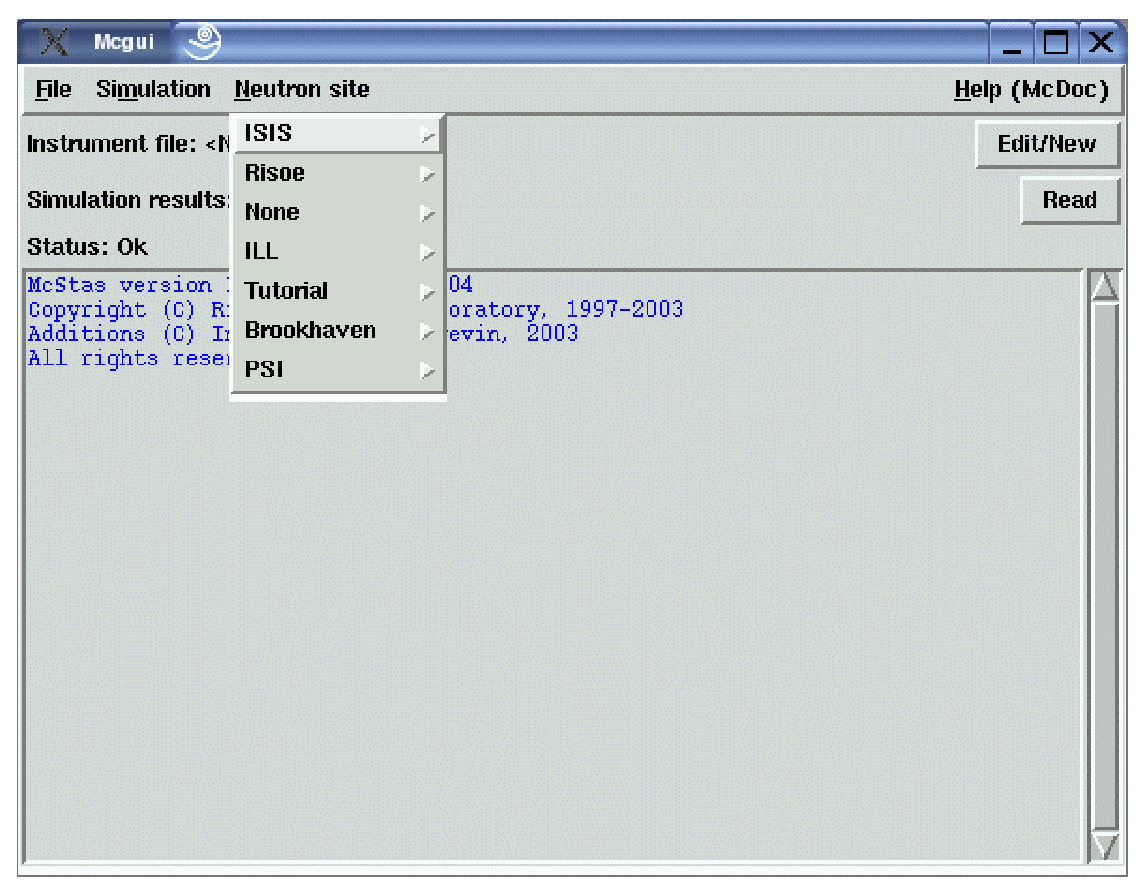
\includegraphics[width=0.55\textwidth]{figures/mcgui.eps}
  \end{center}
\caption{The graphical user interface \texttt{mcgui}.}
\label{fig:mcgui}
\end{figure}

To load an instrument, select ``Open instrument'' from the ``File''
menu. Open the file \verb+vanadium_example.instr+ in the McStas
distribution. Select ``Run simulation'' from the ``Simulation'' menu.
McStas will translate the definition into an executable program and pop
up a dialog window. Type a value for the ``ROT'' parameter ({\em e.g.}
90), check the ``Plot results'' option, and select ``Start''. The
simulation will run, and when it finishes after a while the results will
be plotted in a window.

To debug the simulation graphically, repeat the
steps but check the ``Trace'' option instead of the ``Simulate'' option.
A window will pop up showing a sketch of the instrument.
The left mouse button starts a new neutron, the middle button zooms, and
the right button resets the zoom. The Q key quits the program.

For a slightly longer gentle introduction to McStas, see the McStas
tutorial (available from~\cite{mcstas_webpage}).

\section{Obtaining \MCS}
\label{s:obtain}

The source code for \MCS\ 
%may be obtained from Ris\o{} on a CD-Rom, or it
may be downloaded from the \MCS\ web-page~\cite{mcstas_webpage}, and 
should be available in a file named
\verb+mcstas-+\version\verb+.tar.gz+.
%(the CD-Rom also contains this file under the name
%\verb+mcstas.tgz+ for systems that do not understand long filenames, as
%well as the unpacked sources in the directory \verb+mcstas/+).

The conditions on the use of \MCS\ can be read in the files
\verb+LICENSE+ and \verb+LICENSE.LIB+ in the distribution. Essentially,
\MCS\ may be used and modified freely, but copies of the \MCS\ source code 
may not be distributed to others. 
%We are considering releasing future versions of \MCS\ under a
%more liberal license.
New or modified component and instrument files may, however, be shared by 
the user community.

\subsection{New releases of \MCS}
Releases of new versions of a software can today be carried out more or less
continuously. However, users do not update their software on a daily basis,
and as a compromise we have adopted the following policy of \MCS .

\begin{itemize}
\item A version 1.5.x will contain bug fixes and new functionality. A new manual
will, however, not be released and the modifications are documented on the
\MCS\ web-page. The extensions of the forthcoming version 1.5.x are also listed
on the web, and new versions may be released quite frequently when it is requested
by the user community.
\item A version 1.6 will contain an updated manual. It will typically be released
once or twice a year in connection to for example a \MCS\ workshop.
\item A version 2.0 will hopefully never be released. It would mean that the
code has been rewritten and no backward compability can be expected.
\end{itemize}

\section{Compiling \MCS\ from source}
\label{s:install}

Compilation and installation of \MCS\ contain three
steps. First, the source files must be unpacked:
\begin{verbatim}
    gunzip -c mcstas-1.5.tar.gz | tar xf -
    cd mcstas/
\end{verbatim}
Next, the \verb+configure+ script is run to configure \MCS\ for the
particular machine and operating system, and the software is
compiled:
\begin{verbatim}
    ./configure
    make
\end{verbatim}
Finally, \MCS\ is installed:
\begin{verbatim}
    make install
\end{verbatim}
By default, \MCS\ will be installed in the \verb+usr/local/+ directory
(which typically requires superuser privileges). To install in another
directory, the \verb+--prefix+ option of the \verb+configure+ script can
be used. For example, to install in \verb+/home/joe+ instead:
\begin{verbatim}
    ./configure --prefix=/home/joe
    make
    make install
\end{verbatim}
Depending on which directory \MCS\ is installed in, it may be necessary
to add the \verb+bin/+ subdirectory of the installation directory to the
default path, or to run \MCS\ with the full pathname of the program
(\verb+/usr/local/bin/mcstas+ by default).

The \verb+configure+ command will guess some reasonable defaults for the
C compiler to use. These will be used to compile McStas itself as
well as the simulations produced by McStas. To override\footnote{It may
  be necessary to remove the file \texttt{config.cache} before
  re-installing McStas to have the new settings take effect}
the defaults, the
environment variables \verb+CC+ and \verb+CFLAGS+ can be set to the file
name of the compiler to use and any special compiler options needed (for
example to enable optimization), respectively. After installation, each
user may override the settings using the environment variables
\verb+MCSTAS_CC+ and \verb+MCSTAS_CFLAGS+.

\MCS\ has been tested on x86 Linux, Digital Unix, and HPUX. It should
run on most other Unix-like systems without problems. The main thing to
ensure is that an ANSI-C compliant compiler is available (GCC works
well). If any difficulties arise, the authors should be contacted
so that the problems may be fixed in a later release of \MCS.

To use the \MCS\ front-end programs (see section~\ref{s:frontends}),
certain auxiliary packages must be installed, as described in the README
file in the distribution. These packages are all freely available, and
%have been included on the \MCS\ CD-Rom and on the WWW home page. 
some of
them may be supplied with the operating system (for example,
all required packages are included in Debian/GNU Linux~\cite{debian_webpage}).

Note that the core parts of \MCS, including the \MCS\ compiler and any
generated simulations, work with only
an ANSI-C compiler.


\section{Running the instrument compiler}
\label{s:running}

This section describes how to run the McStas compiler manually. Often,
it will be more convenient to use the front-end program \verb+mcgui+
(section~\ref{s:mcgui}) or \verb+mcrun+ (section~\ref{s:mcrun}). These
front-ends will compile and run the simulations automatically.

The compiler for the \MCS{} instrument definition 
is invoked by typing a command of the form
\begin{verbatim}
    mcstas name.instr
\end{verbatim}
This will read the instrument definition \verb+name.instr+ which is
written in the \MCS\ meta-language. The compiler will translate the
instrument definition into a Monte Carlo simulation program provided in
ANSI-C. The output is by default written to a file in the current
directory with the same name as the instrument file, but with extension
\verb+.c+ rather than \verb+.instr+. This can be overridden using the
\verb+-o+ option as follows:
\begin{verbatim}
    mcstas -o code.c name.instr
\end{verbatim}
which gives the output in the file \verb+code.c+.
A single dash `\verb+-+' may be used for both input and output filename
to represent standard input and standard output, respectively.


\subsection{Code generation options}

By default, the output files from the \MCS\ compiler are in ANSI-C with
some extensions (currently the only extension is the creation of new
directories, which is not possible in pure ANSI-C). The use of
extensions may be disabled with the \verb+-p+ or \verb+--portable+
option. With this option, the output is strictly ANSI-C compliant, at
the cost of some slight reduction in capabilities.

The \verb+-t+ or \verb+--trace+ option puts special ``trace'' code in
the output. This code makes it possible to get a complete trace of the
path of every neutron through the instrument, as well as the position
and orientation of every component. This option is mainly used with the
\verb+mcdisplay+ front-end as described in section~\ref{s:mcdisplay}.

The code generation options can also be controlled by using preprocessor
macros in the C compiler, without the need to re-run the \MCS\
compiler. If the preprocessor macro \verb+MC_PORTABLE+ is defined, the
same result is obtained as with the \verb+--portable+ option of the
\MCS\ compiler. The effect of the \verb+--trace+ option may be obtained
by defining the \verb+MC_TRACE_ENABLED+ macro. Most Unix-like C
compilers allow preprocessor macros to be defined using the \verb+-D+
option, eg.
\begin{verbatim}
    cc -DMC_TRACE_ENABLED -DMC_PORTABLE ...
\end{verbatim}


\subsection{Specifying the location of files}
\label{s:files}

The \MCS\ compiler needs to be able to find various files during
compilation, some explicitly requested by the user (such as component
definitions and files referenced by \verb+%include+),
and some used internally to generate the simulation executable. \MCS\ looks for these
files in three places: first in the current directory, then in a list of
directories given by the user, and finally in a special \MCS\
directory. Usually, the user will not need to worry about this as \MCS\
will automatically find the required files. But if users build their own
component library in a separate directory or if \MCS\ is installed in an
unusual way, it will be necessary to tell the compiler where to look
for the files.

The location of the special \MCS\ directory is set when \MCS\ is
compiled. It defaults to \verb+/usr/local/lib/mcstas+, but it can be
changed to something else, see section~\ref{s:install} for
details. The location can be overridden by setting the environment
variable \verb+MCSTAS+:
\begin{verbatim}
    setenv MCSTAS /home/joe/mcstas
\end{verbatim}
for csh/tcsh users, or
\begin{verbatim}
    export MCSTAS=/home/joe/mcstas
\end{verbatim}
for bash/Bourne shell users.

To make \MCS\ search additional directories for component definitions
and include files, use the \verb+-I+ switch for the \MCS\ compiler:
\begin{verbatim}
    mcstas -I/home/joe/components -I/home/joe/neutron/include name.instr
\end{verbatim}
Multiple \verb+-I+ options can be given, as shown.


\subsection{Embedding the generated simulations in other programs}

By default, \MCS\ will generate a stand-alone C program, which is what
is needed in most cases. However, for advanced usage, such as embedding
the generated simulation in another program or even including two or
more simulations in the same program, a stand-alone program is not
appropriate. For such usage, the \MCS\ compiler provides the following
options:
\begin{itemize}
\item \verb+--no-main+ This option makes \MCS\ omit the \verb+main()+
  function in the generated simulation program. The user must then
  arrange for the function \verb+mcstas_main()+ to be called in some
  way.
\item \verb+--no-runtime+ Normally, the
  generated simulation program contains all the run-time C code necessary for
  declaring functions, variables, etc. used during the simulation.  This
  option makes \MCS\ omit the run-time code from the generated
  simulation program, and the user must then explicitly link with the file
  \verb+mcstas-r.c+ from the \MCS{} distribution.
\end{itemize}
Users that need these options are encouraged to contact the authors for
further help.


\subsection{Running the C compiler}


After the source code for the simulation program has been generated with
the \MCS\ compiler, it must be compiled with the C compiler to produce
an executable. The generated C code obeys the ANSI-C standard, so it
should be easy to compile it using any ANSI-C (or C++) compiler. \textit{E.g}.\ a
typical Unix-style command would be
\begin{verbatim}
    cc -O -o name.out name.c -lm
\end{verbatim}
The \verb+-O+ option typically enables the optimization phase of the compiler,
which can make quite a difference in speed of \MCS\ generated simulations. The
\verb+-o name.out+ sets the name of the generated executable. The \verb+-lm+
options is needed on many systems to link in the math runtime library (like the
$\cos()$ and $\sin()$ functions).

Monte Carlo simulations are computationally intensive, and it is
often desirable to have them run as fast as possible. Some success can
be obtained by adjusting the compiler optimization
options. Here are some example platform and compiler combinations that
have been found to perform well (up-to-date information will be
available on the \MCS\ WWW home page~\cite{mcstas_webpage}):
\begin{itemize}
\item Intel x86 (``PC'') with Linux and GCC, using options \verb+gcc -O3+.
\item Intel x86 with Linux and EGCS (GCC derivate) using
  options \verb+egcc -O6+.
\item Intel x86 with Linux and PGCC (pentium-optimized GCC derivate), using
  options \verb+gcc -O6 -mstack-align-double+.
\item HPPA machines running HPUX with the optional ANSI-C compiler,
  using the options
  \verb|-Aa +Oall -Wl,-a,archive| (the \verb+-Aa+ option is necessary to
  enable the ANSI-C standard).
\end{itemize}
A warning is in place here: it is tempting to spend far more time
fiddling with compiler options and benchmarking than is actually saved
in computation times. Even worse, compiler optimizations are notoriously
buggy; the options given above for PGCC on Linux and the ANSI-C compiler
for HPUX have been known to generate \emph{incorrect code} in some
compiler versions. \MCS\ actually puts an effort into making the task of the C compiler
easier, by in-lining code and using variables in an efficient way. As a
result, \MCS\ simulations generally run quite fast, often fast enough
that further optimizations are not worthwhile.



\section{Running the simulations}
\label{s:run-sim}

Once the simulation program has been generated by the \MCS{} compiler
and an executable has been obtained with the C compiler, the simulation
can be run in various ways. The simplest way is to run it directly from the
command line or shell:
\begin{verbatim}
    ./name.out
\end{verbatim}
Note the leading dot, which is needed if the current directory is not in
the path searched by the shell. When used in this way, the simulation
will prompt for the values of any instrument parameters such as motor
positions, and then run the simulation.  
This way of running \MCS\ will only give data for one spectrometer
setting which is normally sufficient {\em e.g.} for a time-of-flight
spectrometer, but not for a triple-axis spectrometer where a scan over
various spectrometer settings is required.
Often the simulation will be run using one of several
available front-ends, as described in the next section. These front-ends
help manage output from the potentially many detectors in the
instruments, as well as running the simulation for each data point in
a scan.

The generated simulations accept a number of options and arguments. The
full list can be obtained using the \verb+--help+ option:
\begin{verbatim}
    ./name.out --help
\end{verbatim}
The values of instrument parameters may be specified as arguments using
the syntax \textit{name}\verb+=+\textit{val}. For example
\begin{verbatim}
    ./vanadium_example.out ROT=90
\end{verbatim}
The number of neutron histories to simulate may be set using the
\verb+--ncount+ or \verb+-n+ option, for example
\verb+--ncount=2e5+. The initial seed for the random number generator is
by default chosen based on the current time so that it is different for
each run. However, for debugging purposes it is sometimes convenient to
use the same seed for several runs, so that the same sequence of random
numbers is used each time. To achieve this, the random seed may be set
using the \verb+--seed+ or \verb+-s+ option.

By default, \MCS\ simulations write their results into several data
files in the current directory, overwriting any previous files stored
there. The \verb+--dir=+\textit{dir} or \verb+-d+\textit{dir} option
causes the files to be placed instead in a newly created directory
\textit{dir} (to prevent overwriting previous results an error message is given if
the directory already exists). Alternatively, all output may be written
to a single file \textit{file} using the
\verb+--file=+\textit{file} or \verb+-f+\textit{file} option.

By default, data files contain header lines with information about the
simulation from which they originate. In case the data must be analyzed
with programs that cannot read files with such headers, they may be
turned off using the \verb+--ascii-only+ or \verb+-a+ option.

The format of the output files from \MCS\ simulations is described in
more detail in section~\ref{s:analyze}. The complete list of options
and arguments accepted by \MCS\ simulations appears in
table~\ref{f:simoptions}.
\begin{table}
  \begin{center}
    {\let\my=\\
    \begin{tabular}{|p{0.24\textwidth}|p{0.7\textwidth}|}
      \hline
      \texttt{-s {\it seed}} \my \texttt{--seed={\it seed}}
        & Set the initial seed for the random number generator. This may be
        useful for testing to make each run use the same random number
      sequence. \\
      \hline
      \texttt{-n {\it count}} \my \texttt{--ncount={\it count}}
        & Set the number of neutron histories to simulate. The default
      is 1,000,000. \\
      \hline
      \texttt{-d {\it dir}} \my \texttt{--dir={\it dir}}
        & Create a new directory {\it dir\/} and put all data files in
      that directory. \\
      \hline
      \texttt{-f {\it file}} \my \texttt{--file={\it file}}
        & Write all data into a single file {\it file} \\
      \hline
      \texttt{-a} \my \texttt{--ascii-only}
        & Do not put any headers in the data files. \\
      \hline
      \texttt{-h} \my \texttt{--help}
        & Show a short help message with the options accepted, including
        the names of the parameters of the instrument. \\
      \hline
      \texttt{-i} \my \texttt{--info}
        & Show extensive information on the simulation and the
      instrument definition it was generated from. \\
      \hline
      \texttt{-t} \my \texttt{--trace}
        & This option makes the simulation output the state of every
      neutron as it passes through every component. Requires that the
      \texttt{-t} (or \texttt{--trace}) option is also given to the
      \MCS\ compiler when the simulation is generated. \\
      \hline
      \texttt{--no-output-files}
        & This option disables the writing of data files (output to the
      terminal, such as detector intensities, will still be written). \\
      \hline
      \texttt{{\it param}{\texttt =}{\it value}}
        & Set the value of an instrument parameter, rather than having
        to prompt for each one. \\
      \hline
    \end{tabular}
    \caption{Options accepted by \MCS\ simulations}
    \label{f:simoptions}
    }
  \end{center}
\end{table}



\section{Using simulation front-ends}
\label{s:frontends}

\MCS\ includes a number of front-end programs that extend the
functionality of the simulations. The front-end programs is an interface
between the user and the simulations, running the simulations and
presenting the output in various ways to the user.
An extended set of front-end programs is planned for future versions of
\MCS, including a NeXus data format option~\cite{nexus_webpage}.


\subsection{The graphical user interface}
\label{s:mcgui}

The front-end \verb+mcgui+ provides a graphical user interface that
interfaces the various parts of the McStas package. It is started using
simply the command
\begin{verbatim}
    mcgui
\end{verbatim}
The mcgui program may optionally be given the name of an instrument file.

When the front-end is started, a main window is opened. This window
displays the output from compiling and running simulations, and also
contains a few menus and buttons. The main purpose of the front-end is
to edit and compile instrument definitions, run the simulations, and
visualize the results.

\subsubsection{The menus}

The ``File'' menu has the following features:
\begin{description}
\item[Open instrument] selects the name of an instrument file to be used.
\item[Edit current] opens a simple editor window for editing the
  current instrument definition. This function is also available from
  the ``Edit'' button to the right of the name of the instrument definition in
  the main window.
%\item[Spawn editor] This starts the editor defined in the environment
%  variable \verb+VISUAL+ or \verb+EDITOR+ on the current instrument
%  file. It is also possible to start an external editor manually; in any
%  case \verb+mcgui+ will recompile instrument definitions as necessary based on
%  the modification dates of the files on the disk.
\item[Compile instrument] forces a recompile of the instrument
  definition, regardless of file dates. This is for example useful to
  pick up changes in component definitions, which the front-end will not
  notice automatically. See section~\ref{s:install} for how to override
  default C compiler options.
\item[Clear output] erases all text in the window showing output of
  compilations and simulations.
\item[Quit] exits the graphical user interface front-end.
\end{description}

\noindent The ``Simulation'' menu has the following features:
\begin{description}
\item[Read old simulation] prompts for the name of a file
  from a previous run of a McStas simulation (usually called
  \verb+mcstas.sim+). The file will be read and any detector data
  plotted using the \verb+mcplot+ front-end. The parameters used in the
  simulation will also be made the defaults for the next simulation
  run. This function is also available using the ``Read'' button to the
  right of the name of the current simulation data.
\item[Run simulation] opens the run dialog window, explained
  further below.
\item[Plot results] plots (using \verb+mcplot+) the results of the
  last simulation run or loaded.
\end{description}

The ``Help'' menu has a single menu point, ``McStas web-page'', which
attempts to open a Netscape window with the McStas web-page. This
obviously requires that Netscape is properly installed on the computer.


\subsubsection{The run dialog}

\begin{figure}[th]
  \begin{center}
    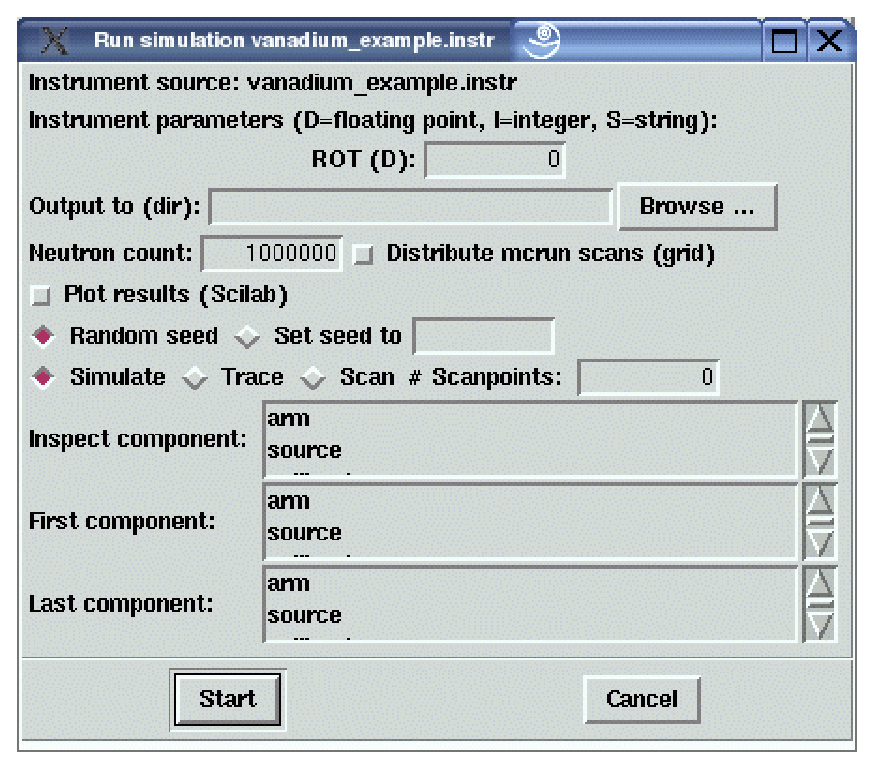
\includegraphics[width=0.45\textwidth]{figures/mcgui-run.eps}
  \end{center}
\caption{The run dialog in \texttt{mcgui}.}
\label{fig:mcgui-run}
\end{figure}
%
The run dialog is used to run simulations. It allows the entry of
instrument parameters as well as the specifications of options for
running the simulation (see section~\ref{s:run-sim} for details). It
also allows to run the \verb+mcdisplay+ (section~\ref{s:mcdisplay}) and
\verb+mcplot+ (section~\ref{s:mcplot}) front-ends together with the
simulation.

The meaning of the different fields is as follows:
\begin{description}
\item[Instrument parameters] allows the setting of the values for
  the input parameters of the instrument. The type of each instrument
  parameter is given in parenthesis after each name. Floating point
  numbers are denoted by (D) (for the C type ``\verb+double+''), (I)
  denotes integer parameters, and (S) denotes strings.
\item[Output to] allows the entry of a directory to store the
  resulting data files in (like the \verb+--dir+ option). If no name is
  given, the results are put in the current directory, to be overwritten
  by the next simulation.
\item[Neutron count] sets the number of neutron histories to
  simulate (the \verb+--ncount+ option).
\item[Plot results] -- if checked, the \verb+mcplot+ front-end will be run
  after the simulation has finished, and the plot dialog will pop up
  (see below).
\item[Random seed/Set seed to] selects between using a random seed (different
  in each simulation) for the random number generator, or using a fixed
  seed (to reproduce results for debugging).
\item[Simulate/Trace] selects between running the simulation
  normally, or using the \verb+mcdisplay+ front-end.
\item[Start] runs the simulation.
\item[Cancel] aborts the dialog.
\end{description}

Before running the simulation, the instrument definition is
automatically compiled if it is newer than the generated C file (or if the C file
is newer than the executable). The executable is
assumed to have a \verb+.out+ suffix in the filename.


\subsubsection{The plot dialog}
\begin{description}
\item[Monitors and detectors] lists all the one- and
  two-dimensional detectors in the instrument. By double-clicking, one plots
  the data in the plot window.
\item[Plot] plots the selected detector in the plot window, just
  like double-clicking its name.
\item[Overview plot] plots all the detectors together in the plot
  window.
\item[B\&W postscript] prompts for a file name and saves the
  current plot as a black and white postscript file. This can
  subsequently be printed on a postscript printer.
\item[Colour postscript] creates a colour postscript file of the
  current plot.
\item[Close] ends the dialog.
\end{description}


\subsubsection{The editor window}

The editor window provides a simple editor for creating and modifying
instrument definitions. Apart from the usual editor functions, the
``Insert'' menu provides some functions that aid in the construction of
the instrument definitions:
\begin{description}
\item[Instrument template] inserts the text for a simple instrument
  skeleton in the editor window.
\item[Component\ldots] opens up a dialog window with a list of all
  the components available for use in McStas. Selecting a component will
  display a description. Double-clicking will open up a dialog window
  allowing the entry of the values of all the parameters for the
  component (figure~\ref{f:comp_dialog}). See section~\ref{s:instrdefs}
  for details of the meaning of the different fields.

The dialog will also pick up those of the users own components that are
  present in the current directory when \verb+mcgui+ is started. See
  section~\ref{s:mcdoc} for how to write components to integrate well
  with this facility.
\item[\textit{Type}] These menu entries give quick access to the entry
  dialog for the various components available.
\end{description}
\begin{figure}[tbp]
  \begin{center}
    \includegraphics[width=0.55\textwidth]{figures/comp_dialog.eps}
    \caption{Component parameter entry dialog.}
    \label{f:comp_dialog}
  \end{center}
\end{figure}


To use the \verb+mcgui+ front-end, the programs Perl, Perl/Tk, PGPLOT, PgPerl,
and PDL must all be properly installed on the system. It may
be necessary to set the \verb+PGPLOT_DIR+ environment variable; consult
the documentation for PGPLOT on the local system in case of difficulty.


\subsection{Running simulations with automatic compilation}
\label{s:mcrun}

The \verb+mcrun+ front-end provides a convenient command-line
interface for running simulations with the same automatic compilation
features available in the \verb+mcgui+ front-end. It also provides a
facility for running a series of simulations while varying an input
parameter, thereby replacing the old \verb+gscan+ front-end.

The command
\begin{quote}
  \texttt{mcrun {\it sim} {\it args\/} \ldots}
\end{quote}
will compile the instrument definition \texttt{{\it sim}.instr} (if
necessary) into an executable simulation \texttt{{\it sim}.out}. It
will then run \texttt{{\it sim}.out}, passing the argument list {\it
  args}

The possible arguments are the same as those accepted by the simulations
themselves as described in section~\ref{s:run-sim}, with the following
extensions:
\begin{itemize}
\item The \verb+-c+ or \verb+--force-compile+ option may be used to for
  the recompilation of the instrument definition, regardless of file
  dates. This may be needed in case any component definitions are
  changed (in which case \verb+mcrun+ does not automatically recompile),
  or if a new version of McStas has been installed.
\item The \texttt{-p {\it file}} or \texttt{--param={\it file}} option
  may be used to specify a file containing assignment of values to the
  input parameters of the instrument definition. The file should consist
  of specifications of the form \texttt{{\it name\/}={\it value\/}}
  separated by spaces or line breaks. Multiple \verb+-p+ options may be
  given together with direct parameter specifications on the command
  line. If a parameter is assigned multiple times, later assignments
  override previous ones.
\item The \texttt{-N {\it count}} or \texttt{--numpoints={\it count}} option
  may be used to perform a series of \textit{count\/} simulations while
  varying one or more parameters within specified intervals. Such a
  series of simulations is called a \emph{scan}. To specify
  an interval for a parameter \textit{X}, it should be assigned two
  values separated with a comma. For example, the command
\begin{verbatim}
    mcrun sim.instr -N4 X=2,8 Y=1
\end{verbatim}
would run the simulation defined in \verb+sim.instr+ four times, with
\textit{X} having the values 2, 4, 6, and 8, respectively.

After running the simulation, the results will be written to the file
\verb+mcstas.dat+ by default. This file contains one line for each
simulation run giving the values of the scanned input variables along
with the intensity and estimated error in all detectors. Additionally, a
file \verb+mcstas.sim+ is written that can be read by the \verb+mcplot+
front-end to plot the results on the screen or in a Postscript file, see
section~\ref{s:mcplot}.
\item When doing a scan, the \texttt{-f {\it file}} and
  \texttt{--file={\it file}} options make \verb+mcrun+ write the output
  to the files \texttt{{\it file\/}.dat} and \texttt{{\it file\/}.sim}
  instead of the default names.
\item When doing a scan, the \texttt{-d {\it dir}} and
  \texttt{--dir={\it dir}} options make \verb+mcrun+ put all output in a
  newly created directory \textit{dir}. Additionally, the directory will
  have subdirectories \verb+1+, \verb+2+, \verb+3+,\ldots containing all
  data files output from the different simulations. When the \verb+-d+
  option is not used, no data files are written from the individual
  simulations (in order to save disk space).
\end{itemize}

The \verb+mcrun+ front-end requires a working installation of Perl to run.


\subsection{The \texttt{gscan} front-end}
\label{gscan}

The front-end \verb+gscan+ is obsolete from version~1.3 of McStas, and
is included only for backwards compatibility. The front-end~\verb+mcrun+
(section~\ref{s:mcrun}) includes all the functionality of the old
\verb+gscan+ front-end and should be used instead.


\subsection{Graphical display of simulations}
\label{s:mcdisplay}

The front-end \verb+mcdisplay+ is a graphical debugging tool.
It presents a schematic drawing of the instrument
definition, showing the position of the components and the paths of the
simulated neutrons through the instrument. It is thus very useful for
debugging a simulation, for example to spot components in the wrong
position or to find out where neutrons are getting lost. The graphics
is shown on an X Windows display.

To use the \verb+mcdisplay+ front-end with a simulation, run it as
follows:
\begin{quote}
  \verb+mcdisplay sim.out +{\it args \ldots}
\end{quote}
where \verb+sim+ is the name of the simulation program generated with
\MCS\ and \textit{args \ldots} are the normal command line arguments for
the simulation, as explained above. 
This will view the instrument from above. A
multi-display that shows the instrument from three directions
simultaneously can be shown using the \verb+--multi+ option:
\begin{quote}
  \verb+mcdisplay --multi sim.out +{\it args \ldots}
\end{quote}
The \verb+mcdisplay+ front-end can also be run from the \verb+mcgui+ front-end.

Click the left mouse button in the graphics window or hit the space key
to see the display of successive neutron trajectories. The `P' key saves
a postscript file containing the current display that can be sent to the
printer to obtain a hardcopy; the `C' key produces color postscript. 
To stop the simulation
prematurely, type `Q' or use control-C as normal in the window in which
\verb+mcdisplay+ was started.

To see details in the instrument, it is possible to zoom in on a part of
the instrument using the middle mouse button (or the `Z' key on systems
with a one- or two-button mouse). The right mouse button (or the `X'
key) resets the zoom. Note that after zooming, the units on the
different axes may no longer be equal, and thus the angles as seen on
the display may not match the actual angles.

Another way to see details while maintaining an overview of the
instrument is to use the \verb+--zoom=+\textit{factor} option. This
magnifies the display of each component along the selected axis only,
{\em e.g.} a Soller collimator is magnified perpendicular to the neutron beam
but not along it. This option may produce rather strange visual effects
as the neutron passes between components with different coordinate
magnifications, but it is occasionally useful.

When debugging, it is often the case that one is interested only in
neutrons that reach a particular component in the instrument. For
example, if there is a problem with the sample one may prefer not to see
the neutrons that are absorbed in the monochromator shielding. For these
cases, the \verb+--inspect=+\textit{comp\/} option is useful. With this
option, only neutrons that reach the component named \textit{comp\/} are
shown in the graphics display.

See section~\ref{s:comp-mcdisplay} for how to make new components work
with the \verb+mcdisplay+ front-end. The \verb+mcdisplay+ front-end
requires the Perl, the PGPLOT, and the PGPerl packages to be installed.


\subsection{Plotting the results of a simulation}
\label{s:mcplot}

The front-end \verb+mcplot+ is a program that produces
plots of all the detectors in a simulation, and it is thus useful to get
a quick overview of the simulation results.

In the simplest case, the front-end is run simply by typing
\begin{verbatim}
    mcplot
\end{verbatim}
This will plot any simulation data stored in the current directory,
which is where simulations put their results by default. If the
\verb+--dir+ or \verb+--file+ options have been used (see
section~\ref{s:run-sim}), the name of the file or directory should be
passed to mcplot, {\em e.g.} ``\texttt{mcplot {\it dir}}'' or ``\texttt{mcplot
  {\it file}}''.

The initial display shows plots for each detector in the simulation.
Clicking the left mouse button on a plot produces a full-window version
of that plot. The `P' key saves a postscript file containing the current
plot that can be sent to the printer to obtain a hardcopy; the `C' key
produces color postscript. 
The `Q' key quits the program (or CTRL-C in the controlling
terminal may be used as normal).

To use the \verb+mcplot+ front-end, the programs Perl, PGPLOT, PgPerl,
and PDL must all be properly installed on the system.



\subsection{Plotting resolution functions}
\label{s:mcresplot}

The \verb+mcresplot+ front-end is used to plot the resolution function
of a triple-axis 
%or inverse geometry time-of-flight 
spectrometer, as
calculated by the Res\_sample component. 
%(see section~\ref{s:res_sample}). 
This front-end 
has been included in the release since it may be useful
despite its somewhat rough user interface.

The \verb+mcresplot+ front-end is run with the command
\begin{quote}
  \texttt{mcresplot {\it file\/}}
\end{quote}
Here, {\it file\/} is the name of a file output from a simulation using
the Res\_monitor component.
% (section~\ref{s:res_monitor}). 
The front-end
will open two windows. One shows a three-dimensional visualization of
the resolution function using the two components of $\boldsymbol{Q}$ in
the scattering plane and $\omega$. The plot may be rotated using the
mouse while pressing the left button, and zoomed while pressing the
right button.

The other window displays the covariance matrix of the resolution
function and the resulting resolution matrix. This is mainly useful for
triple-axis spectrometers. The four bottom plots visualize the
covariance matrix using four different projections. The top left corner
shows histograms of the resolution function along the three axes of
$\boldsymbol{Q}$ and along the $\omega$ axis.

Pressing the ``Q'' key while the three-dimensional window is active
switches to a combined plot where the yellow dots show the resolution
function and the red dots show the covariance matrix. A second press of
the ``Q'' key ends the front-end program.

To use the \verb+mcresplot+ front-end, the programs Perl, PGPLOT, PgPerl,
and PDL must all be properly installed on the system.



\section{Analyzing and visualizing the simulation results}
\label{s:analyze}

To analyze simulation results, one uses the same tools as for analyzing
experimental data, \textit{i.e}. programs such as the MATLAB packages
Mview and Mfit %\cite{mfit} 
used at Ris\o. The output files from
simulations are simply columns of ASCII text that most programs should
be able to read. A future version of \MCS\ will support output in the
NeXus format~\cite{nexus_webpage}.

One-dimensional histogram detectors (time-of-flight, energy-sensitive)
write one line for each histogram bin. Each line contains a number
identifying the bin (\textit{i.e}.\ the time-of-flight) followed by
three numbers: the simulated intensity, an estimate of the statistical
error as explained in section~\ref{s:staterror}, and the number of
neutron events for this bin.

Two-dimensional histogram detectors (position sensitive detectors)
output $M$ lines of $N$ numbers representing neutron intensities, where
$M$ and $N$ are the number of bins in the two dimensions. The
two-dimentional detectors do not store any error estimates since this is
seldom useful, however if needed it can be obtained using
\verb+MC_GETPAR+ in the \verb+FINALLY+ section of the instrument
definition, see section~\ref{s:comp-declare}.

Single-point detectors output the neutron intensity, the estimated
error, and the neutron event count as numbers on the
terminal. (The results from a series of simulations may be combined in a
data file using the \verb+mcrun+ front-end as explained in
section~\ref{s:mcrun}).

Both one- and two-dimentional detector output by default start with a
header of comment lines, all beginning with the `\verb+#+' character.
This header gives such information as the name of the instrument used in
the simulation, the values of any instrument parameters, the name of the
detector component for this data file, \textit{etc}. The headers may be
disabled using the \verb+--ascii-only+ option in case the file must be
read by a program that cannot handle the headers.

In addition to the files written for each one- and two-dimensional
detector component, another file (by default named \verb+mcstas.sim+) is
also created. This file is in a special \MCS\ ASCII format. It contains
all available information about the instrument definition used for the
simulation, the parameters and options used to run the simulation, and
the detector components present in the instrument. It is read by the
\verb+mcplot+ front-end (see section~\ref{s:mcplot}). This file stores
the results from single detectors, but by default contains only pointers
(in the form of file names) to data for one- and two-dimensional
detectors. By storing data in separate files, reading the data with
programs that do not know the special \MCS\ file format is
simplified. The \verb+--file+ option may be used to store all data
inside the \verb+mcstas.sim+ file instead of in separate files.

Note that the neutron event counts in detectors is typically not very
meaningful except as a way to measure the performance of the
simulation. Use the simulated intensity instead whenever analysing
simulation data.

% Emacs settings: -*-mode: latex; TeX-master: "manual.tex"; -*-

\chapter{The \MCS\ kernel and meta-language}
\label{s:kernel}
\index{Kernel|textbf}

Instrument definitions are written in a special \MCS\ meta-language which
is translated automatically by the \MCS\ compiler into a C program 
which is in turn compiled to an executable that
performs the simulation. The meta-language is custom-designed for neutron
scattering and serves two main purposes: (i) to specify the interaction of a
single neutron with a single optical component, and (ii) to build a
simulation by constructing a complete instrument from individual
components.

For maximum flexibility and efficiency, the meta-language is based on C.
Instrument geometry, propagation of neutrons between the different
components, parameters, data input/output etc.\ is handled in the
meta-language and by the \MCS\ compiler. Complex calculations are written in
C embedded in the meta-language description of the components. It is
possible to set up an instrument from existing components and
run a simulation without writing a single line of C code, working
entirely in the meta-language. On the other hand, the full power of the C
language is available for special-purpose setups in advanced
simulations, and for computing neutron trajectories in the components.

Apart from the meta-language, \MCS\ also includes a number of C library
functions and definitions that are useful for neutron ray-tracing
simulations. The definitions available for users coding components are
listed in appendix~\ref{c:kernelcalls}. The list includes functions for
computing the intersection between a flight-path and various objects
(such as cylinders and spheres), functions for generating random numbers
with various distributions, functions for reading or writing
informations from/to data files, convenient conversion
factors between relevant units, etc. \index{Library!Run-time}
\index{Library!Components!share}

The \MCS\ meta-language was designed to be readable, with a verbose
syntax and explicit mentioning of otherwise implicit information. The
recommended way to get started with the meta-language is to start by
looking at the examples supplied with \MCS, modifying them as necessary
for the application at hand.

\section{Notational conventions}

Simulations generated by \MCS\ use a semi-classical description of the
neutron to compute the neutron trajectory through the instrument and its
interaction with the different components. The effect of gravity is
taken  into account either in particular components, or more generaly
when setting an execution flag (\verb+-g+) to perform gravitation
computation. \index{Gravitation}

An instrument consists of a list of components through which the neutron
passes one after the other. The order of components is thus significant
since \MCS\ does not automatically check which component is the next to
interact with the neutron at a given point in the simulation.

The instrument is given a global, absolute coordinate system. In
addition, every component in the instrument has its own local coordinate
system that can be given any desired position and orientation (though
the position and orientation must remain fixed for the duration of a
single simulation). \index{Coordinate system}
By convention, the $z$ axis points in the direction of the beam, the $x$ axis
is perpendicular to the beam in the horizontal plane pointing left as seen
from the source, and the $y$ axis points upwards (see figure~\ref{f:axis}).
Nothing in \MCS\ enforces this convention, but if every component used
different conventions the user would be faced with a severe headache! It is
therefore recommended that this convention is followed by users implementing
new components.
\begin{figure}
  \begin{center}
    \includegraphics[width=0.8\textwidth]{figures/axis-conventions.eps}
  \end{center}
\caption{conventions for the orientations of the axis in simulations.}
\label{f:axis}
\end{figure}

\index{Neutron state and units}
In the instrument definitions, units of length (\textit{e.g}.\ component
positions) are given in meters and units of angles (\textit{e.g}.\ 
rotations) are given in degrees.  The state of the neutron is given by
its position $(x,y,z)$ in meters, its velocity $(v_x, v_y, v_z)$ in
meters per second, the time $t$ in seconds, and the two parameters
  %\footnote{The
  %spin is ignored in the current version 1.4 of \MCS. However, while not
  %documented in this manual, preliminary support for components that
  %handle the neutron spin is implemented using the POLARISATION
  %PARAMETER construct. We are currently working together with Trefor
  %Roberts at the ILL to get a correct handling of the spin.} 
$s_1$ and $s_2$ that are obsolete and should not be used. A three-component
representation of the spin, $\left( s_x, s_y, s_z \right)$, normalized to
one, is used. In addition, the outgoing neutron has an associated weight $p$
which is used to model fractional neutrons in the Monte Carlo simulation.
$p=0.2$ means that a single neutron following this path has a 20\% chance of
reaching the present position without being absorbed or scattered away from
the instrument. Alternatively, one may regard a ray of neutrons and $p$ is
the fraction of neutrons following the considered path.

\section{Syntaxical conventions}
\label{s:syntax}

Comments follow the normal C syntax ``\verb+/* ... */+''. C++ style
comments ``\verb+// ...+'' may also be used.
\index{Comments}

%For backward-compatibility
%with early versions, comments may also be written as a percentage sign
%followed by a space (``\verb*+% ...+''), but this is not recommended and
%will be removed in a future version.

Keywords are not case-sensitive, for example ``\verb+DEFINE+'',
``\verb+define+'', and ``\verb+dEfInE+'' are all equivalent. However, by
convention we always write keywords in uppercase to distinguish them
from identifiers and C language keywords. In contrast, \MCS\ 
identifiers (names), like C identifiers and keywords, \emph{are} case
sensitive, another good reason to use a consistent case convention for
keywords. All \MCS\ keywords are reserved, and thus should not be used 
as C variable names. The list of these reserved keywords is shown in table~\ref{t:keywords}. \index{Keyword}

\begin{table}
  \begin{center} 
    {\let\my=\\
    \begin{tabular}{|l|c|p{0.7\textwidth}|}
      \hline
      \texttt{Keyword} & Scope & Meaning \\
      \hline
      \texttt{ABSOLUTE} & I & Indicates that the AT and ROTATED keywords are in the absolute coordinate system. \\
      \texttt{AT} & I & Indicates the position of a component in an instrument definition. \\
      \texttt{DECLARE} & I,C & Declares C internal instrument or component variables. \\
      \texttt{DEFINE} & I,C & Starts an instrument or component definition. \\
      \texttt{- INSTRUMENT} & & (each associated parameter may have default values) \\
      \texttt{- COMPONENT} & & \\
      \texttt{DEFINITION} & C & Defines component parameters that are constants (like C \#define). \\
      \texttt{END} & I,C & Ends the instrument or component definition. \\
      \texttt{EXTEND} & I & Extends the TRACE section of a component in an instrument definition. \\
      \texttt{FINALLY} & I,C & Embeds C code to execute when simulation ends (also executes the SAVE section). \\
      \texttt{GROUP} & I & Defines an exclusive group of components. \\
      \texttt{\%include} & I,C & Imports an instrument part, a component or a piece of C code (when within embedded C). \\
      \texttt{INITIALIZE} & I,C & Embeds C code to be executed when starting. \\
      \texttt{MCDISPLAY} & C & Embeds C code to display a geometric  representation of a component. \\
      \texttt{OUTPUT} & C & Defines internal variables to be public and protected symbols (usually all those of DECLARE).\\
      \texttt{PARAMETERS} & C & Defines a class of component parameter. \\
      \texttt{POLARISATION} & C & Defines neutron polarisation coordinates. \\
      \texttt{PREVIOUS} & C & Refers to a previous component position/orientation.\\
      \texttt{RELATIVE} & I & Indicates that the AT and ROTATED keywords are relative to an other component. \\
      \texttt{ROTATED} & I & Indicates the orientation of a component in an instrument definition. \\
      \texttt{SAVE} & I,C & Embedded C code to execute when saving data. \\
      \texttt{SETTING} & C & Defines component parameters that are
      variables (double, int, char*). \\
      \texttt{SHARE} & C & Declares global functions and variables to be used by all components. \\
      \texttt{STATE} & C & Defines neutron state coordinates. \\
      \texttt{TRACE} & I,C & Lists the components or embedded C code to execute during simulation. \\
      \hline
    \end{tabular}
    \caption{Reserved \MCS\ keywords. 
    Scope is 'I' for instrument and 'C' for component definitions.}
    \label{t:keywords}
    }
  \end{center}
\end{table}

It is possible, and usual, to split the input instrument definition
across several different files. For example, if a component is not
explicitly defined in the instrument,
\MCS\ will search for a file containing the component definition in the
standard component library (as well as in the current directory and any
user-specified search directories, see section~\ref{s:files}). It is
also possible to explicitly include another file using a line of the
form \index{Keyword!\%include}
\begin{verbatim}
    %include "file"
\end{verbatim}
Beware of possible confusion with the C language ``\verb+#include+''
statement, especially when it is used in C code embedded within the
\MCS\ meta-language. Files referenced with ``\verb+%include+'' are read
when the instrument is translated into C by the \MCS\ compiler, and must
contain valid \MCS\ meta-language input (and possibly C code). Files referenced with
``\verb+#include+'' are read when the C compiler generates an
executable from the generated C code, and must contain valid C.

Embedded C code is used in several instances in the \MCS\
meta-language. Such code is copied by the \MCS\ compiler into the
generated simulation C program. Embedded C code is written by putting it
between the special symbols \verb|%{| and \verb|%}|, as follows:
\begin{quote}
  \verb|%{| \\
  \hbox to 3em{}\ldots Embedded C code \ldots \\
  \verb|%}|
\end{quote} \index{Embedded C code}
The ``\verb|%{|'' and ``\verb|%}|'' must appear on a line by themselves (do not add comments after).
Additionally, if a ``\verb+%include+'' statement is found \emph{within} an embedded C code block, the specified file will be included from the 'share' directory of the standard component library \index{Library!Components!share} (or from the
current directory and any user-specified search directories) as a C library, just like the usual ``\verb+#include+'' \emph{but only once}. For instance, if many components require to read data from a file, they may all ask for ``\verb+%include "read_table-lib"+'' \index{Library!read\_table-lib (Read\_Table)} without duplicating the code of this library. If the file has no extension, both \verb+.h+ and \verb+.c+ files will be searched and included, otherwise, only the specified file will be imported. The \MCS\ 'run-time' shared 
library is included by default (equivalent to ``\verb+%include "mcstas-r"+'' in the \texttt{DECLARE} section). \index{Library!Run-time}
For an
example of \texttt{\%include}, see the monitors/Monitor\_nD component.


\section{Writing instrument definitions}
\label{s:instrdefs}
\index{Instruments}

The purpose of the instrument definition is to specify a sequence of
components, along with their position and parameters, which together
make up an instrument. Each component is given its own local coordinate
system, the position and orientation of which may be specified by its
translation and rotation relative to another component. An example is
given in section~\ref{s:vanadium_example.instr} and some additional
examples of instrument definitions can be found on the McStas
web-page~\cite{mcstas_webpage} and in the \texttt{example} directory.

%An instrument definition looks as follows:


\subsection{The instrument definition head}

\begin{quote}
  \texttt{DEFINE} \texttt{INSTRUMENT} \textit{name} $(a_1, a_2, \ldots)$
\end{quote} \index{Keyword!DEFINE!INSTRUMENT}
This marks the beginning of the definition. It also gives the name of
the instrument and the list of instrument parameters. Instrument
parameters describe the configuration of the instrument, and usually
correspond to setting parameters of the components. A motor position is
a typical example of an instrument parameter. The input parameters of
the instrument constitute the input that the user (or possibly a
front-end program) must supply when the
generated simulation is started. 

\index{Parameters!Instruments}
By default, the parameters will be floating point numbers, and will have
the C type \verb+double+ (double precision floating point). The type of
each parameter may optionally be declared to be \verb+int+ for the C
integer type or \verb+char *+ for the C string type. The name
\verb+string+ may be used as a synonym for \verb+char *+, and floating
point parameters may be explicitly declared using the name
\verb+double+. The following example illustrates all possibilities:
\begin{quote}
  \texttt{DEFINE INSTRUMENT test(d1, double d2, int i, char *s1, string s2)}
\end{quote}
Here \verb+d1+ and \verb+d2+ will be floating point parameters of C type
\verb+double+, \verb+i+ will be an integer parameter of C type
\verb+int+, and \verb+s1+ and \verb+s2+ will be string parameters of C
type \verb+char *+. 
\index{Parameters!Optional, default value}
The parameters of an instrument may be given default values. Parameters with default values are called \emph{optional
  parameters}, and need not be given an explicit value when the
instrument simulation is executed. When executed without any parameter value in the command line (see section~\ref{s:run-sim}), the instrument asks for all parameter values, but pressing the \verb+Return+ key selects the default value (if any). When used with at least one parameter value in the command line, all non specified parameters will have their value set to the default one (if any). A parameter is given a
default value using the syntax ``\textit{param}\texttt{ = }\textit{value}''.
For example
\begin{quote}
  \texttt{DEFINE INSTRUMENT test(d1 = 1, string s2="hello")}
\end{quote}
Here \verb+d1+ is an optional parameter and if no value is given
explicitly, ``1'' will be used.

Optional parameters can greatly increase the convenience for users of
instruments for which some parameters are seldom changed or of unclear signification to the user. Also, if all instrument parameters have default values, then the simple command \verb+mcdisplay+ \verb+test.instr+ will show the instrument view without requesting any other input, which is usually a good starting point to study the instrument design.

\subsection{The \texttt{DECLARE} section}
\index{Keyword!DECLARE}
\label{s:declare}

\begin{quote}
  \texttt{DECLARE} \\
  \verb|%{| \\
  \hbox to 3em{}\ldots C declarations of global variables etc. \ldots \\
  \verb|%}|
\end{quote} \index{Embedded C code}
This gives C declarations that may be referred to in the rest of the
instrument definition. A typical use is to declare global variables or
small functions that are used elsewhere in the instrument. The \verb+%include ''file''+ keyword may be used to import a specific
component definition or a part of an instrument. The \texttt{DECLARE} section is optional.

\subsection{The \texttt{INITIALIZE} section}
\index{Keyword!INITIALIZE}
\label{s:initialize}

\begin{quote}
  \texttt{INITIALIZE} \\
  \verb|%{| \\
  \hbox to 3em{}\ldots C initializations. \ldots \\
  \verb|%}|
\end{quote} \index{Embedded C code}
This gives code that is executed when the simulation starts. This section is
optional.


\subsection{The \texttt{TRACE} section}
\index{Keyword!TRACE}
\label{s:trace}

The \texttt{TRACE} keyword starts a section giving the list of
components that constitute the instrument.
Components are declared like this:
\begin{quote}
  \texttt{COMPONENT} $\textit{name} =
    \textit{comp}(p_1 = e_1, p_2 = e_2, \ldots)$
\end{quote}
\index{Components}
\index{Keyword!COMPONENT} \index{Parameters!Setting}
\index{Parameters!Definition}
This declares a component named \textit{name} that is an instance of the
component definition named \textit{comp}. The parameter list gives the
setting and definition parameters for the component. The expressions $e_1,
e_2, \ldots$ define the values of the parameters. For setting parameters
arbitrary ANSI-C expressions may be used, while for definition parameters
only \emph{constant} numbers, strings, names of instrument parameters, or names
of C identifiers are allowed (see section~\ref{s:comp-header} for details of
the difference between definition and setting parameters). To assign the
value of a general expression to a definition parameter, it is necessary to
declare a variable in the \texttt{DECLARE} section, assign the value to the
variable in the \texttt{INITIALIZE} section, and use the variable as the
value for the parameter.

The \MCS\ program takes care to rename parameters appropriately in the
output so that no conflicts occur between different component
definitions or between component and instrument definitions. It is thus
possible (and usual) to use a component definition multiple times
in an instrument description.

The \MCS\ compiler will automatically search for a file containing a
definition of the component if it has not been declared previously. The
definition is searched for in a file called ``{\it name\/}{\tt .comp}'',
``{\it name\/}{\tt .cmp}'', or ``{\it name\/}{\tt .com}''. See
section~\ref{s:files} for details on which directories are searched. This
facility is often used to refer to existing component definitions in
standard component libraries. It is also possible to write component
definitions in the main file before the instrument definitions, or to
explicitly read definitions from other files using \verb+%include+ 
(not within embedded C blocks).

The position of a component is specified using an \texttt{AT} modifier
following the component declaration:
\index{Keyword!AT} \index{Keyword!RELATIVE} \index{Keyword!ABSOLUTE}
\begin{quote}
  \texttt{AT} $(x,y,z)$ \texttt{RELATIVE} \textit{name}
\end{quote}
This places the component at position $(x,y,z)$ in the coordinate system
of the previously declared component \textit{name}. Placement may also
be absolute (not relative to any component) by writing
\begin{quote}
  \texttt{AT} $(x,y,z)$ \texttt{ABSOLUTE}
\end{quote}
Any C expression may be used for $x$, $y$, and $z$. The \texttt{AT}
modifier is required.
Rotation is achieved similarly by writing \index{Keyword!ROTATED}
\begin{quote}
  \texttt{ROTATED} $(\phi_x,\phi_y,\phi_z)$ \texttt{RELATIVE} \textit{name}
\end{quote}
This will result in a coordinate system that is rotated first the angle
$\phi_x$ (in degrees) around the $x$ axis, then $\phi_y$ around the $y$ axis, and finally
$\phi_z$ around the $z$ axis. Rotation may also be specified using
\texttt{ABSOLUTE} rather than \texttt{RELATIVE}. If no rotation is
specified, the default is $(0,0,0)$ using the same relative or absolute
specification used in the \texttt{AT} modifier. The \emph{position} of a component depends on its definition. Usually, it will be the input window position (e.g. for guide-like components), or the center position for cylindrical/spherical components. Thus, the next component position will be most of the time set to the previous component AT position increased by its size/radius along the $z$ axis.

The \texttt{PREVIOUS} \index{Keyword!PREVIOUS} keyword is a generic name to refer to the previous component in the simulation. Moreover, the \texttt{PREVIOUS(n)} keyword will refer to the $n$-th previous component, starting from the current component, so that \texttt{PREVIOUS} is equivalent to \texttt{PREVIOUS(1)}. This keyword should be used after the \texttt{RELATIVE} keyword, but not for the first component instance of the instrument description.
\begin{quote}
  \texttt{AT} $(x,y,z)$ \texttt{RELATIVE} \texttt{PREVIOUS}
  \texttt{ROTATED} $(\phi_x,\phi_y,\phi_z)$ \texttt{RELATIVE} \texttt{PREVIOUS(2)}
\end{quote}
Invalid \texttt{PREVIOUS} references will be assumed to be absolute placement. 

The order and position of components in the \texttt{TRACE} section does not
allow components to overlap, except for particular cases (see the \texttt{GROUP} keyword below).
Indeed, many components of the \MCS\ library \index{Library!Components} start
by propagating the neutron event to the begining of the component itself.
Anyway, when the corresponding propagation time is found to be negative
({\it i.e.} the neutron is already \emph{after} the component, and has thus
passed the 'active' position), the neutron event is ABSORBed, resulting in a zero intensity and event counts after a given position. Such situations
may arise e.g. when positioning some components not one after the other (nested, in parallel, or overlapping), for
instance in a multiple crystal monochromator (they are then side by side). One
would then like the neutron to interact with \emph{one of} the components and
then continue after this group of components. In order to handle such
arrangements, groups are defined by appending the \texttt{GROUP} modifier
\begin{quote}
  \texttt{GROUP} \textit{name}
\end{quote}
to all involved component declarations. \index{Keyword!GROUP}
All components of the same named group are tested one after the other, until one of them interacts (uses the SCATTER macro \index{Library!Run-time!SCATTER}). The selected component acts on the neutron, and the rest of the group is skipped. Such groups are thus exclusive (only one of the elements is active).
If no component of the group could intercept the neutron, it is ABSORBed. If you wish not to absorb these neutrons, you may end each group by a large monitor, which will eventually catch neutrons that were not caught by previous components of the group.

It is sometimes desirable to slighlty modify an existing component of the \MCS\ library. One would usually make a copy of the component, and extend the code of its \texttt{TRACE} section. \MCS\ provides an easy way to change the behaviour of existing components in an instrument definition without duplicating files, using the \texttt{EXTEND} modifier \index{Keyword!EXTEND}
\begin{quote}
  \texttt{EXTEND} \\
  \verb|%{| \\
  \hbox to 3em{}\ldots C code executed after the component TRACE section \ldots \\
  \verb|%}|
\end{quote} \index{Embedded C code}
The embeded C code is appended to the component \texttt{TRACE} section, and all its internal variables (as well as all the instrument variables) may be used.
This component declaration modifier is of course optional. Within a \texttt{GROUP}, \emph{all} \texttt{EXTEND} sections of the group are executed. In order to discriminate components that are active from those that are skipped, one may use the SCATTERED flag, which is set to zero when entering each component or group, and incremented when the neutron is SCATTERed, as in the following example \index{Library!Run-time!SCATTER} \index{Library!Run-time!SCATTERED}
\begin{quote}
  \texttt{COMPONENT} $\textit{name0} =
    \textit{comp}(p_1 = e_1, p_2 = e_2, \ldots)$ \\
  \hbox to 1em{} \texttt{AT} $(0,0,0)$ \texttt{ABSOLUTE} \\
  \texttt{COMPONENT} $\textit{name1} =
    \textit{comp}(\ldots)$ \\
  \hbox to 1em{} \texttt{AT} $(x,y,z)$ \texttt{RELATIVE} \textit{name0} \\
  \hbox to 1em{} \texttt{ROTATED} $(\phi_x,\phi_y,\phi_z)$ \texttt{RELATIVE} \textit{name0} \\
  \hbox to 1em{} \texttt{GROUP} \textit{GroupName} \texttt{EXTEND} \\
  \hbox to 1em{} \verb|%{| \\
  \hbox to 3em{} \verb+if (SCATTERED) printf("I scatter"); else printf("I do not scatter");+\\
  \hbox to 1em{} \verb|%}| \\
  \texttt{COMPONENT} $\textit{name2} =
    \textit{comp}(\ldots)$ \\
  \hbox to 1em{} \texttt{AT} $(x,y,z)$ \texttt{RELATIVE} \textit{name0} \\
  \hbox to 1em{} \texttt{ROTATED} $(\phi_x,\phi_y,\phi_z)$ \texttt{RELATIVE} \textit{name0} \\
  \hbox to 1em{} \texttt{GROUP} \textit{GroupName}
\end{quote}
Components \emph{name1} and \emph{name2} are at the same position. If the first one intercepts the neutron (and has a SCATTER within its \texttt{TRACE} section), the SCATTERED variable becomes true, the code extension will result in printing "I scatter", and the second component will be skipped.
Thus, we recommand to make use of the SCATTER keyword each time a component 'uses' the neutron (scatters, detects, \ldots).


\subsection{The \texttt{SAVE} section}
\index{Keyword!SAVE}
\label{s:save}

\begin{quote}
  \texttt{SAVE} \\
  \verb|%{| \\
  \hbox to 3em{}\ldots C code to execute each time a temporary save is required \ldots \\
  \verb|%}|
\end{quote} \index{Signal handler!USR2 signal}
This gives code that will be executed when the simulation is requested to save data, for instance when receiving a USR2 signal (on Unix systems), or using the \verb+Progress_bar+ component with intermediate savings. This section is optional.

\subsection{The \texttt{FINALLY} section}
\index{Keyword!FINALLY}
\label{s:finally}

\begin{quote}
  \texttt{FINALLY} \\
  \verb|%{| \\
  \hbox to 3em{}\ldots C code to execute at end of simulation \ldots \\
  \verb|%}|
\end{quote}
This gives code that will be executed when the simulation has
ended. When existing, the \texttt{SAVE} section is first executed. This section is optional.
A simulation may be requested to end before all neutrons have been traced when recieving a TERM or INT signal (on Unix systems), or with Control-C.
\index{Signal handler!TERM signal} \index{Signal handler!INT signal}


\subsection{The end of the instrument definition}
\label{s:end}
\index{Keyword!END}

The end of the instrument definition is marked using the keyword
\begin{quote}
  \texttt{END}
\end{quote}

\subsection{Code for the instrument \texttt{vanadium\_example.instr}}
\label{s:vanadium_example.instr}
An instrument definition taken from the \texttt{examples} directory is
given as an example.
\smallverbatimfile{../mcstas/lib/examples/vanadium_example.instr}

\section{Writing component definitions}
\label{s:compdefs}

The purpose of a component definition is to model the interaction of a
neutron with the component. Given the state of the incoming neutron, the
component definition calculates the state of the neutron when it leaves
the component.  The calculation of the effect of the component on the
neutron is performed by a block of embedded C code. 
One example of a component definition is given in section~\ref{s:slit}, and all
component definitions can be found on the McStas web-page~\cite{mcstas_webpage}.

There exists a large number of functions and constants available in
order to write efficient components. Look at the appendix~\ref{c:kernelcalls} for neutron propagation functions, geometric intersection time computations, vector operators, random number and vector generation, physical constants, coordinate retrieval and operations, file generation routines (for monitors), data file reading, \ldots

%A component definition looks as follows:


\subsection{The component definition header}
\label{s:comp-header}

\begin{quote}
  \texttt{DEFINE} \texttt{COMPONENT} \textit{name}
\end{quote}
\index{Keyword!DEFINE!COMPONENT}
This marks the beginning of the definition, and defines the name of the
component.
\begin{quote}
  \texttt{DEFINITION} \texttt{PARAMETERS} $(d_1, d_2, \ldots)$ \\
  \texttt{SETTING} \texttt{PARAMETERS} $(s_1, s_2, \ldots)$
\end{quote}
\index{Keyword!DEFINITION PARAMETERS}
\index{Keyword!SETTING PARAMETERS}
This declares the definition and setting parameters of the component.
The parameters define the characteristics of the component, and can be
accessed from the \verb+SAVE+, \verb+FINALLY+, and \verb+MCDISPLAY+ sections (see below), 
as well as in \verb+EXTEND+ sections of the instrument definition (see section~\ref{s:instrdefs}).
\index{Parameters!Setting}
\index{Parameters!Definition}

Setting parameters are translated into C variables usually of type
\verb+double+ in the generated simulation program, so they are usually
numbers. Definition parameters are translated into \verb+#define+ macro
definitions, and so can have any type, including strings, arrays, and
function pointers.

However, because of the use of \verb+#define+, definition parameters
suffer from the usual problems with C macro definitions. Also, it is not
possible to use a general C expression for the value of a definition
parameter in the instrument definition, only constants and variable
names may be used. For this reason, setting parameters should be used
whenever possible.

There are a few cases where the use of definition parameters instead of
setting parameters makes sense. If the parameter is not numeric, nor a character string ({\em i.e.} an
array, for example), a setting parameter cannot be
used. Also, because of the use of \verb+#define+, the C compiler can
treat definition parameters as constants when the simulation is
compiled. For example, if the array sizes of a multidetector are
definition parameters, the arrays can be statically allocated in the
component \verb+DECLARE+ section. If setting parameters were used, it
would be necessary to allocate the arrays dynamically using {\em e.g.}\ 
\verb+malloc()+.

Setting parameters may optionally be declared to be of type \verb+int+ and \verb+char *+, just as in the instrument definition (see section~\ref{s:instrdefs}).

\begin{quote}
  \texttt{OUTPUT} \texttt{PARAMETERS} $(s_1, s_2, \ldots)$
\end{quote}
\index{Keyword!OUTPUT PARAMETERS}
This declares a list of C identifiers that are output parameters for the
component. Output parameters are used to hold values that are computed
by the component itself, rather than being passed as input. This could
for example be a count of neutrons in a detector or a constant that is
precomputed to speed up computation. Output
parameters will typically be declared as C variables in the
\texttt{DECLARE} section, see section~\ref{s:comp-declare} below for an
example.

The \texttt{OUTPUT} \texttt{PARAMETERS} section is optional.

\begin{quote}
  \texttt{STATE} \texttt{PARAMETERS} $(x,y,z,v_x,v_y,v_z,t,s_1,s_2,p)$
\end{quote}
\index{Keyword!STATE PARAMETERS}
This declares the parameters that define the state of the incoming
neutron. The task of the component code is to assign new values to these
parameters based on the old values and the values of the definition and
setting parameters. Note that $s_1$ and $s_2$ are obsolete and cannot be used.

\begin{quote}
  \texttt{POLARISATION} \texttt{PARAMETERS} $(s_x,s_y,s_z)$
\end{quote}
\index{Keyword!POLARISATION PARAMETERS}
This line is necessary only if the component handles polarisation of neutrons
and thus modifies the spin vector. For an instrument to handle polarisation
correctly, it is only required that {\em one} of the components contains this
line.

\subsubsection{Optional component parameters}
\index{Parameters!Optional, default value}

Just as for instrument parameters, the definition and setting parameters of a
component may be given a default value. Parameters with default values are
called \emph{optional parameters}, and need not be given an explicit value when
the component is used in an instrument definition. A parameter is given a
default value using the syntax ``\textit{param}\texttt{ = }\textit{value}''.
For example
\begin{quote}
  \texttt{SETTING PARAMETERS (radius, height, pack = 1)}
\end{quote}
Here \verb+pack+ is an optional parameter and if no value is given
explicitly, ``1'' will be used\footnote{In contrast, if no value is
  given for \texttt{radius} or \texttt{height}, an error message will
  result.}.

Optional parameters can greatly increase the convenience for users of
components with many parameters that have natural default values which
are seldom changed. Optional parameters are also useful to preserve
backwards compatibility with old instrument definitions when a component
is updated. New parameters can be added with default values that
correspond to the old behavior, and existing instrument definitions can
be used with the new component without changes.

However, optional parameters should not be used in cases where no
general natural default value exists. For example, the length of a guide
or the size of a slit should not be given default values. This would
prevent the error messages that should be given in the common case of a
user forgetting to set an important parameter.


\subsection{The \texttt{DECLARE} section}
\label{s:comp-declare}
\begin{quote}
  \texttt{DECLARE} \\
  \verb|%{| \\
  \hbox to 3em{}\ldots C code declarations (variables, definitions, functions)\ldots \\
  \hbox to 3em{}\ldots These are usually OUTPUT parameters to avoid name conflicts \ldots \\
  \verb|%}|
\end{quote}
\index{Keyword!DECLARE}
This gives C declarations of global variables etc. that are used by the
component code. This may for instance be used to declare a neutron
counter for a detector component. This section is optional.

Note that any variables declared in a \verb+DECLARE+ section are
\emph{global}. Thus a name conflict may occur if two instances of a
component are used in the same instrument. To avoid this, variables
declared in the \texttt{DECLARE} section should be \texttt{OUTPUT} parameters of
the component because \MCS\ will then rename variables to avoid conflicts. 
For example, a simple detector might be defined as follows:
\begin{quote}
\begin{verbatim}
DEFINE COMPONENT Detector
OUTPUT PARAMETERS (counts)
DECLARE
%{
  int counts;
%}
...
\end{verbatim}
\end{quote}
\index{Keyword!OUTPUT PARAMETERS}
\index{Library!Run-time!MC\_GETPAR}
The idea is that the \texttt{counts} variable counts the number of
neutrons detected. In the instrument definition, the \texttt{counts}
parameter may be referenced using the \verb+MC_GETPAR+ C macro, as in
the following example instrument fragment:\label{mcgetpar}
\begin{quote}
\begin{verbatim}
COMPONENT d1 = Detector()
...
COMPONENT d2 = Detector()
...
FINALLY
%{
  printf("Detector counts: d1 = %d, d2 = %d\n",
         MC_GETPAR(d1,counts), MC_GETPAR(d2,counts));
%}
\end{verbatim}
\end{quote}

\subsection{The \texttt{SHARE} section}
\label{s:comp-share}
\begin{quote}
  \texttt{SHARE} \\
  \verb|%{| \\
  \hbox to 3em{}\ldots C code \emph{shared} declarations (variables, definitions, functions)\ldots \\
  \hbox to 3em{}\ldots These should not be OUTPUT parameters \ldots \\
  \verb|%}|
\end{quote}
\index{Keyword!SHARE}

The \texttt{SHARE} section has the same role as \texttt{DECLARE} except that when using more than one instance of the component, it is inserted \emph{only once} in the simulation code. No occurence of the items to be shared should be in the \texttt{OUTPUT} parameter list (not to have \MCS\ rename the identifiers). 
This is particularly useful when using many instances of the same component (for instance guide elements). If the declarations were in the \texttt{DECLARE} section, \MCS\ would duplicates it for each instance (making the simulation code bigger).
A typical example is to have shared variables, functions, type and structure definitions that may be used from the component \texttt{TRACE} section. For an
example of \texttt{SHARE}, see the samples/Single\_crystal
component. The \verb+%include ''file''+ keyword may be used to import
a shared library. The \texttt{SHARE} section is optional.

\subsection{The \texttt{INITIALIZE} section}
\label{s:comp-initialize}

\begin{quote}
  \texttt{INITIALIZE} \\
  \verb|%{| \\
  \hbox to 3em{}\ldots C code initialization \ldots \\
  \verb|%}|
\end{quote}
\index{Keyword!INITIALIZE}
This gives C code that will be executed once at the start of the
simulation, usually to initialize any variables declared in the
\texttt{DECLARE} section. This section is optional.


\subsection{The \texttt{TRACE} section}
\label{s:comp-trace}

\begin{quote}
  \texttt{TRACE} \\
  \verb|%{| \\
  \hbox to 3em{}\ldots C code to compute neutron interaction with
    component \ldots \\
  \verb|%}|
\end{quote}
\index{Keyword!TRACE}
This performs the actual computation of the interaction between the neutron
and the component. The C code should perform the appropriate
calculations and assign the resulting new neutron state to the state
parameters.

\index{Library!Run-time!ABSORB}
The C code may also execute the special macro \texttt{ABSORB} to indicate
that the neutron has been absorbed in the component and the simulation of
that neutron will be aborted. When the neutron state is changed or detected, for
instance if the component simulates multiple events (for example multiple
reflections in a guide, or multiple scattering in a powder sample), the
special macro \texttt{SCATTER} should be called. This does not affect the
results of the simulation in any way, but it allows the front-end
programs to visualize the scattering events properly, and to handle
component \texttt{GROUP}s in an instrument definition (see
section~\ref{s:trace}). The \texttt{SCATTER} macro should be called with
the state parameters set to the proper values for the scattering event.
For an example of \texttt{SCATTER}, see the optics/Channeled\_guide
component. \index{Library!Run-time!SCATTER}


\subsection{The \texttt{SAVE} section}
\label{s:comp-save}
\index{Data format}
\index{Keyword!SAVE}

\begin{quote}
  \texttt{SAVE} \\
  \verb|%{| \\
  \hbox to 3em{}\ldots C code to execute in order to save data \ldots \\
  \verb|%}|
\end{quote}
This gives code that will be executed when the simulation is requested to save data, for instance when receiving a USR2 signal (on Unix systems, see section~\ref{s:run-sim}), or when triggered by the \texttt{Progress\_bar(flag\_save=1)} component.
This might be used by monitors and detectors in order to write results.
An extension depending on the selected output format (see~\ref{t:formatoptions} and section~\ref{s:run-sim}) is automatically appended to file names, if these latter do not contain extension.

In order to work properly with the common output file format used in
\MCS, all monitor/detector components should use standard macros for
outputting data in the SAVE or FINALLY section, as explained below. In the
following, we use $N = \sum_i p_i^0$ to denote the count of detected
neutron events, $p = \sum_i p_i$ to denote the sum of the weights of
detected neutrons, and $\textit{p2} = \sum_i p_i^2$ to denote the sum of
the squares of the weights, as explained in section~\ref{s:staterror}.

\paragraph{Single detectors/monitors}
\label{s:DETECTOR_OUT}
\index{Library!Run-time!DETECTOR\_OUT}

The results of a single detector/monitor are written using the following
macro:
\begin{quote}
  \texttt{DETECTOR\_OUT\_0D({\it t}, $N$, $p$, {\it p2})}
\end{quote}
Here, \textit{t} is a string giving a short descriptive title for the
results, {\em e.g.}\ ``Single monitor''.


\paragraph{One-dimensional detectors/monitors}

The results of a one-dimensional detector/\discretionary{}{}{}mon\-i\-tor are written using the
following macro:
\begin{quote}
  \texttt{DETECTOR\_OUT\_1D({\it t},
        {\it xlabel},
        {\it ylabel},
        {\it xvar}, $x_{\rm min}$, $x_{\rm max}$, $m$, \\
        \phantom{\texttt{DETECTOR\_OUT\_1D(}}% Paren hack ->)
          $\&N[0]$, $\&p[0]$, $\&{\it p2}[0]$,
        {\it filename})}
\end{quote}
Here,
\begin{itemize}
\item \textit{t} is a string giving a descriptive title ({\em e.g.}\ ``Energy
  monitor''),
\item \textit{xlabel} is a string giving a descriptive label for the X
  axis in a plot ({\em e.g.}\ ``Energy [meV]''),
\item \textit{ylabel} is a string giving a descriptive label for the Y
  axis of a plot ({\em e.g.}\ ``Intensity''),
\item \textit{xvar} is a string giving the name of the variable on the X
  axis ({\em e.g.}\ ``E''),
\item $x_{\rm min}$ is the lower limit for the X axis,
\item $x_{\rm max}$ is the upper limit for the X axis,
\item $m$ is the number of elements in the detector arrays,
\item $\&N[0]$ is a pointer to the first element in the array of $N$
  values for the detector component (or NULL, in which case no error
  bars will be computed),
\item $\&p[0]$ is a pointer to the first element in the array of $p$
  values for the detector component,
\item $\&{\it p2}[0]$ is a pointer to the first element in the array of
  {\it p2} values for the detector component (or NULL, in which case no error
  bars will be computed),
\item \textit{filename} is a string giving the name of the file in which
  to store the data.
\end{itemize}


\paragraph{Two-dimensional detectors/monitors}

The results of a two-dimensional detector/\discretionary{}{}{}mon\-i\-tor are written to a file using the
following macro:
\begin{quote}
  \texttt{DETECTOR\_OUT\_2D({\it t},
        {\it xlabel},
        {\it ylabel},
        $x_{\rm min}$, $x_{\rm max}$, $y_{\rm min}$, $y_{\rm max}$, $m$, $n$,\\
        \phantom{\texttt{DETECTOR\_OUT\_2D(}}% Paren hack ->)
          $\&N[0][0]$, $\&p[0][0]$, $\&{\it p2}[0][0]$,
        {\it filename})}
\end{quote}
Here,
\begin{itemize}
\item \textit{t} is a string giving a descriptive title ({\em e.g.}\ ``PSD
  monitor''),
\item \textit{xlabel} is a string giving a descriptive label for the X
  axis in a plot ({\em e.g.}\ ``X position [cm]''),
\item \textit{ylabel} is a string giving a descriptive label for the Y
  axis of a plot ({\em e.g.}\ ``Y position [cm]''),
\item $x_{\rm min}$ is the lower limit for the X axis,
\item $x_{\rm max}$ is the upper limit for the X axis,
\item $y_{\rm min}$ is the lower limit for the Y axis,
\item $y_{\rm max}$ is the upper limit for the Y axis,
\item $m$ is the number of elements in the detector arrays along the X axis,
\item $n$ is the number of elements in the detector arrays along the Y axis,
\item $\&N[0][0]$ is a pointer to the first element in the array of $N$
  values for the detector component,
\item $\&p[0][0]$ is a pointer to the first element in the array of $p$
  values for the detector component,
\item $\&{\it p2}[0][0]$ is a pointer to the first element in the array of
  {\it p2} values for the detector component,
\item \textit{filename} is a string giving the name of the file in which
  to store the data.
\end{itemize}
Note that for a two-dimensional detector array, the first dimension is
along the X axis and the second dimension is along the Y axis. This
means that element $(i_x,i_y)$ can be obtained as $p[i_x*n+i_y]$ if $p$
is a pointer to the first element.

\paragraph{Three-dimensional detectors/monitors}

The results of a three-dimensional detector/\discretionary{}{}{}mon\-i\-tor are written to a file using the
following macro:

\begin{quote}
  \texttt{DETECTOR\_OUT\_3D({\it t},
        {\it xlabel}, {\it ylabel}, {\it zlabel},
        {\it xvar}, {\it yvar}, {\it zvar},
        $x_{\rm min}$, $x_{\rm max}$, $y_{\rm min}$, $y_{\rm max}$, 
        $z_{\rm min}$, $z_{\rm max}$, $m$, $n$, $p$\\
        \phantom{\texttt{DETECTOR\_OUT\_3D(}}% Paren hack ->)
          $\&N[0][0][0]$, $\&p[0][0][0]$, $\&{\it p2}[0][0][0]$,
        {\it filename})}
\end{quote}
The meaning of parameters is the same as those used in the 1D and 2D
versions of DETECTOR\_OUT. The available data format currently save
the 3D arrays as 2D, with the 3rd dimension specified in the {\it
  type} field of the data header.

\subsection{The \texttt{FINALLY} section}
\label{s:comp-finally}
\index{Keyword!FINALLY}

\begin{quote}
  \texttt{FINALLY} \\
  \verb|%{| \\
  \hbox to 3em{}\ldots C code to execute at end of simulation \ldots \\
  \verb|%}|
\end{quote}
This gives code that will be executed when the simulation has
ended. This might be used to free memory and print out final results from components, \textit{e.g}.\ the
simulated intensity in a detector.

\subsection{The \texttt{MCDISPLAY} section}
\label{s:comp-mcdisplay}
\index{Keyword!MCDISPLAY}

\begin{quote}
  \texttt{MCDISPLAY} \\
  \verb|%{| \\
  \hbox to 3em{}\ldots C code to draw a sketch of the component \ldots \\
  \verb|%}|
\end{quote}
This gives C code that draws a sketch of the component in the plots
produced by the \verb+mcdisplay+ front-end (see
section~\ref{s:mcdisplay}). The section can contain arbitrary C code and
may refer to the parameters of the component, but usually it will
consist of a short sequence of the special commands described below that
are available only in the MCDISPLAY section.
When drawing components, all distances and positions are in meters and
specified in the local coordinate system of the component.

The MCDISPLAY section is optional. If it is omitted, \verb+mcdisplay+
will use a default symbol (a small circle) for drawing the component.

\paragraph{The {\tt magnify} command}

This command, if present, must be the first in the section. It takes a
single argument: a string containing zero or more of the letters ``x'',
``y'' and ``z''. It causes the drawing to be enlarged along the
specified axis in case \verb+mcdisplay+ is called with the \verb+--zoom+
option. For example:
\begin{verbatim}
    magnify("xy");
\end{verbatim}


\paragraph{The {\tt line} command}

The {\tt line} command takes the following form:
\begin{quote}
  \texttt{line($x_1$, $y_1$, $z_1$, $x_2$, $y_2$, $z_2$)}
\end{quote}
It draws a line between the points $(x_1, y_1, z_1)$ and $(x_2, y_2,
z_2)$.


\paragraph{The {\tt multiline} command}

The {\tt multiline} command takes the following form:
\begin{quote}
  \texttt{multiline($n$, $x_1$, $y_1$, $z_1$, ..., $x_n$, $y_n$, $z_n$)}
\end{quote}
It draws a series of lines through the $n$ points $(x_1, y_1, z_1)$,
$(x_2, y_2, z_2)$, \ldots, $(x_n, y_n, z_n)$. It thus accepts a variable
number of arguments depending on the value of $n$. This exposes 
one of the nasty quirks of C since \emph{no} type checking is
performed by the C compiler. It is thus very important that all
arguments to {\tt multiline} (except $n$) are valid numbers of type {\tt
  double}. A common mistake is to write
\begin{verbatim}
    multiline(3, x, y, 0, ...)
\end{verbatim}
which will silently produce garbage output. This must instead be
written as
\begin{verbatim}
    multiline(3, (double)x, (double)y, 0.0, ...)
\end{verbatim}


\paragraph{The {\tt circle} command}

The {\tt circle} command takes the following form:
\begin{quote}
  \texttt{circle({\it plane}, $x$, $y$, $z$, $r$)}
\end{quote}
Here {\it plane} should be either \verb+"xy"+, \verb+"xz"+, or
\verb+"yz"+. The command draws a circle in the specified plane with the center
 at $(x, y, z)$ and the radius $r$.



\subsection{The end of the component definition}
\index{Keyword!END}

\begin{quote}
  \texttt{END}
\end{quote}
This marks the end of the component definition.

\subsection{A component example: Slit}
\label{s:slit}
A simple example of the component \texttt{Slit} is given.

\smallverbatimfile{../mcstas/lib/optics/Slit.comp}


\subsection{McDoc, the McStas library documentation tool}
\label{s:mcdoc}
\index{Tools!mcdoc}

%From version 1.3, 
McStas includes a facility called McDoc to help maintain good documentation of
components and instruments. In the component source code, comments may be
written that follow a particular format understood by McDoc. The McDoc facility
will read these comments and automatically produce output documentation in
various forms. By using the source code itself as the source of documentation,
the documentation is much more likely to be a faithful and up-to-date
description of how the component/instrument actually works.

%In McStas version 1.4, 
Two forms of documentation can be generated. One
is the component entry dialog in the \verb+mcgui+ front-end, see
section~\ref{s:mcgui}. The other is a collection of web pages documenting
the components and instruments, handled via the \verb+mcdoc+ front-end (see section~\ref{s:mcdoc-run}), and the complete documentation for all available
McStas components and instruments may be found at the \MCS\
webpage~\cite{mcstas_webpage}, and in the \MCS\ library (see~\ref{s:comp-overview}). This latter is accessible from the \verb+mcgui+ 'Help' menu.

Note that McDoc-compliant comments in the source code are no substitute
for a good reference manual entry. The mathematical equations describing
the physics and algorithms of the component should still be written up
carefully for inclusion in the component manual. The McDoc comments are
useful for describing the general behaviour of the component, the
meaning and units of the input parameters, etc.


\subsubsection{The format of the comments in the library source code}

The format of the comments understood by McDoc is mostly
straight-forward, and is designed to be easily readable both by humans
and by automatic tools. McDoc has been written to be quite tolerant in
terms of how the comments may be formatted and broken across lines. A
good way to get a feeling for the format is to study some of the examples
in the existing components and instruments. Below, a few
notes are listed on the requirements for the comment headers:

The comment syntax uses \verb+%IDENTIFICATION+, \verb+%DESCRIPTION+,
\verb+%PARAMETERS+, \verb+%LINKS+, and \verb+%END+
keywords to mark different sections of the documentation. Keywords may
be abbreviated, \textit{e.g.} as \verb+%IDENT+ or \verb+%I+.

\begin{itemize}
\item In the \verb+%IDENTIFICATION+
  section, \verb+author:+ (or \verb+written by:+ for backwards
  compatibility with old comments) denote author; \verb+date:+,
  \verb+version:+, and \verb+origin:+ are also supported. Any number of
  \verb+Modified by:+ entries may be used to give the revision history.
  The \verb+author:+, \verb+date:+, etc. entries must all
  appear on a single line of their own. Everything else in the
  identification section is part of a "short description" of the
  component.
\item In the \verb+%PARAMETERS+
  section, descriptions have the form
  \hbox{``\texttt{{\it name\/}:~[{\it unit\/}] {\it text\/}}''}
  or \hbox{``\texttt{{\it name\/}:~{\it text\/} [{\it unit\/}]}''}.
  These may span multiple lines, but subsequent lines must be
  indented by at least four spaces. Note that square brackets \verb+[]+ should
  be used for units. Normal parenthesis are also supported for backwards
  compatibility, but nested parenthesis do not work well.
\item The \verb+%DESCRIPTION+
  section contains text in free format. The text may contain HTML tags
  like \verb+<IMG>+ (to include pictures) and
  \verb+<A>+\ldots\verb+</A>+
  (for links to other web pages, but see also the \verb+%LINK+
  section). In the generated web documentation pages, the text is set in
  \verb+<PRE>+\ldots\verb+</PRE>+, so that the line breaks in the source
  will be obeyed.
\item Any number of \verb+%LINK+
  sections may be given; each one contains HTML code that will be put in
  a list item in the link section of the description web page. This
  usually consists of an \verb+<A HREF="..."> ... </A>+ pointer to some
  other source of information.
\item Optionally, an \verb+%INSTRUMENT_SITE+ section followed by a single word is used to sort \emph{instruments} by origin/location in the 'Neutron Site' menu in \verb+mcgui+.
\item After \verb+%END+, no more comment text is read by McDoc.
\end{itemize}

\include{comp_abstract}
\include{instrum}
%% Emacs settings: -*-mode: latex; TeX-master: "manual.tex"; -*-

\chapter{Test results}
\label{testresults}

In this Appendix, we present a few illustrative
results from the three instruments presented in 
section \ref{s:instrument}. A more thorough presentation
may be found on the \MCS\ home page \cite{mcstas_webpage}.

\section{Scattering from the V-sample test instrument}
\label{s:vanadium-result}

In figure \ref{f:V-results}, we present the radial distribution 
of the scatting from an evenly illuminated V-sample,
as seen by a spherical PSD.
It is interesting to note that the variation in the
scattering intensity is as large as 10\%. This is an effect
of attenuation of the beam in the cylindrical sample.

\begin{figure}
  \begin{center}
    \includegraphics[width=0.6\textwidth]{vanadium-surf-2.eps}
  \end{center}
\caption{Scattering from a V-sample, measured by a spherical
  PSD. The sphere has been transformed onto a plane and the intensity is
  plotted as the third dimension. A colour version of this picture is
  found on the title page of this manual.}
\label{f:V-results}
\end{figure}

\section{Simulated and measured resolution of TAS1}
\label{data:TAS1}

In order to test the \MCS\ package on a qualitative level,
we have performed a very detailed simulation of the conventional
triple axis spectrometer TAS1, Ris\o . The measurement series
constitutes a complete alignment of the spectrometer,
using the direct beam and scattering from V and Al$_2$O$_3$
samples at an incoming energy of 20.0~meV, using the second order
scattering from the monochromator. 
In the instrument definitions, we have used all available
information about the spectrometer. However, the
mosaicities of the monochromator and analyser are set
to 45' in stead of the quoted 30', since we from our
analysis believe this to be much closer to the truth.

In these simulations, we have tried to reproduce
every alignment scan with respect to position and width
of the peaks, whereas we have not tried to compare
absolute intensities. Below, we show a few comparisons 
of the simulations and the measurements. 

Figure \ref{f:2t_direct} shows a scan of 
$2\theta_s$ on the collimated direct beam in two-axis mode.
A 1 mm slit is placed on the sample position.
Both the measured width and non-Gaussian peak shape
are well reproduced by the \MCS\ simulations.

\begin{figure}
  \begin{center}
    \includegraphics[width=0.6\textwidth]{tas1-2T.eps}
  \end{center}
\caption{Scans of $2\theta_s$ in the direct beam with 1 mm slit on the
  sample position.
"$\times$": measurements, "o": simulations  
Collimations: open-30'-open-open.}
\label{f:2t_direct}
\end{figure}

In contrast, a simulated $2\theta_a$ scan in triple-axis 
mode on a V-sample showed a surprising offset from zero, see
Figure \ref{f:v_2ta_offset}. However, a simulation with a PSD
on the sample position showed that the beam center was 1.5~mm
off from the center of the sample, and this was important
since the beam was no wider than the sample itself.
A subsequent centering of the beam resulted in a nice
agreement between simulation and measurements. 
For a comparison on a slightly different instrument
(analyser-detector collimator inserted), 
see Figure~\ref{f:v_2ta_zero}.

\begin{figure}
  \begin{center}
    \includegraphics[width=0.6\textwidth]{vanadium-plot-1.eps}
  \end{center}
\caption{First simulated $2\theta_a$ scan on a vanadium sample.
Collimations: open-30'-28'-open.}
\label{f:v_2ta_offset}
\end{figure}

\begin{figure}
  \begin{center}
    \includegraphics[width=0.6\textwidth]{vanadium-plot-2.eps}
  \end{center}
\caption{Corrected $2\theta_a$ scan on a V-sample.
Collimations: open-30'-28'-67'.
"$\times$": measurements, "o": simulations.}
\label{f:v_2ta_zero}
\end{figure}

The result of a $2\theta_s$ scan on an Al$_2$O$_3$
powder sample in two-axis mode is shown in Figure \ref{f:al2o3}.
Both for the scan in focusing mode (+ $-$ +)
and for the one in defocusing mode (+ + +) (not shown),
the agreement between simulation and experiment is excellent.

\begin{figure}
  \begin{center}
    \includegraphics[width=0.6\textwidth]{al2o3-focus.eps}
  \end{center}
\caption{$2\theta_s$ scans on Al$_2$O$_3$ in two-axis, focusing mode.
Collimations: open-30'-28'-67'.
"$\times$": measurements, "o": simulations.  
A constant background is added to the simulated data.}
\label{f:al2o3}
\end{figure}

As a final result, we present a scan of the energy
transfer $E_a = \hbar \omega$ on a V-sample.
The data are shown in Figure \ref{f:v_ea}.

\begin{figure}
  \begin{center}
    \includegraphics[width=0.6\textwidth]{ea-scan.eps}
  \end{center}
\caption{Scans of the analyser energy on a V-sample.
Collimations: open-30'-28'-67'.
"$\times$": measurements, "o": simulations.}
\label{f:v_ea}
\end{figure}


\section{Simple spectra from the PRISMA instrument}
\label{data:PRISMA}

A plot from the detector in the PRISMA simulation is shown in Figure
\ref{f:PRISMAdata}. These results were obtained with each analyser blade
rotated one degree relative to the previous one. The separation of the
spectra of the different analyser blades is caused by different energy
of scattered neutrons and different flight path length from source to
detector.  We have not performed any quantitative analysis of the data at this
time.

\begin{figure}
  \begin{center}
    \includegraphics[width=0.6\textwidth]{prisma2-a.eps}
  \end{center}
\caption{Test result from PRISMA instrument using ``coloured
  neutrons''. Each graph shows the neutrons scattered from one analyser blade.}
\label{f:PRISMAdata}
\end{figure}

   % now in instrum
%% Emacs settings: -*-mode: latex; TeX-master: "manual.tex"; -*-

\chapter{Planned expansions of \MCS\ in the future}
\label{future}

During the work so far on
\MCS, we have run across a number of points we would like to
include in \MCS\ in the future.

For the \MCS\ meta-language itself, these points include:
\begin{itemize}
\item Facilities for making a Monte-Carlo choice on the basis of 
tabulated values. This would be useful in source and filter components.
\item Facilities for assembling a number of existing components into one
compound component, like a multi-bladed analyser.
\end{itemize}
We also would like to improve on the component and instrument libraries:
\begin{itemize}
\item Output in NeXus format.
\item Allow multiple scattering in sample components.
\item More samples for inelastic scattering.
\item A powder sample with more than one reflection.
\item Handle gravitation.
\item The RITA spectrometer.
\item The new Ris\o\ TAS7 spectrometer.
\item A detailed version of the ISIS PRISMA spectrometer.
\end{itemize}
Further, we would like to make improvements on the interface software:
\begin{itemize}
\item Interface to existing control software ({\em e.g.} the Ris\o{}
  program TASCOM)
\end{itemize}
 % now in changes

\appendix
%\include{tutorial}
%\include{polarisation}
\include{random}
% Emacs settings: -*-mode: latex; TeX-master: "manual.tex"; -*-

\chapter{Kernel calls and conversion constants}
\label{c:kernelcalls}
The \MCS\ kernel contains a number of built-in functions
and conversion constants which are useful when constructing
components. Here, we present a short list of these features.

\section{Kernel calls and functions}
Here we list a number of preprogrammed macros 
which may ease the task of writing component and instrument definitions.

\subsection{Neutron propagation}
\begin{itemize}
\item {\bf ABSORB}. This macro issues an order to the overall
  \MCS\ simulator to interrupt the simulation of the current neutron
  history and to start a new one.
\item {\bf PROP\_Z0}. Propagates the neutron to the $z=0$ plane,
  by adjusting $(x,y,z)$ and $t$. If the neutron velocity 
  points away from the $z=0$ plane, the neutron is absorbed.
\item {\bf PROP\_DT}$(dt)$. Propagates the neutron through the
  time interval $dt$, adjusting $(x,y,z)$ and $t$.
\item {\bf PROP\_GRAV\_DT}$(dt,Ax,Ay,Az)$. Like {\bf PROP\_DT}, but it also
  includes gravity using the acceleration $(Ax,Ay,Az)$. In addition,
  to adjusting $(x,y,z)$ and $t$ also $(vx,vy,vz)$ is modified.
\item {\bf SCATTER}. This macro is used to denote a scattering event
  inside a component, see section~\ref{s:comp-trace}.
\end{itemize}

\subsection{Meta-language extensions}
\begin{itemize}
\item {\bf MC\_GETPAR}(). This may be used in the finally section of an
  instrument definition to reference the output parameters of a
  component. See page~\pageref{mcgetpar} for details.
\item {\bf NAME\_CURRENT\_COMP} gives the name of the current component as a string.
\item {\bf POS\_A\_CURRENT\_COMP} gives the absolute position of the 
  current component. A component of the vector is referred to as
  {\bf POS\_A\_CURRENT\_COMP.i} where $i$ is $x$, $y$ or $z$.
\item {\bf ROT\_A\_CURRENT\_COMP} and 
  {\bf ROT\_R\_CURRENT\_COMP} give the orientation
  of the current component as rotation matrices
  (absolute orientation and the orientation relative to
  the previous component, respectively). A
  component of a rotation matrice is referred to as 
  {\bf ROT\_A\_CURRENT\_COMP[m][n]}, where $m$ and
  $n$ are 0, 1, or 2.
\item {\bf POS\_A\_COMP(comp)} gives the absolute position
  of the component with the name {\em comp}. Note that
  {\em comp} is not given as a string. A component of the
  vector is referred to as {\bf POS\_A\_COMP(comp).i}
  where $i$ is $x$, $y$ or $z$.
\item {\bf ROT\_A\_COMP(comp)} and
  {\bf ROT\_R\_COMP(comp)} give the orientation of the
  component {\em comp} as rotation matrices (absolute
  orientation and the orientation relative to its
  previous component, respectively). Note that {\em comp}
  is not given as a string. A component of  a rotation
  matrice is referred to as 
  {\bf ROT\_A\_COMP(comp)[m][n]}, where $m$ and $n$ are
  0, 1, or 2. 
\item {\bf extend\_list}($n$, \&\textit{arr}, \&\textit{len},
  \textit{elemsize}). Given an array \textit{arr} with \textit{len}
  elements each of size \textit{elemsize}, make sure that the array is
  big enough to hold at least $n$ elements, by extending \textit{arr}
  and \textit{len} if necessary. Typically used when reading a list of
  numbers from a data file when the length of the file is not known in advance.
\item {\bf mcget\_ncount}(). Returns the number of neutron histories to simulate.
\end{itemize}

\subsection{Mathematical routines}
\begin{itemize}
\item {\bf NORM}$(x,y,z)$. Normalizes the vector $(x,y,z)$ to have
  length 1.
\item {\bf scalar\_prod}$(a_x,a_y,a_z,b_x,b_y,b_z)$. Returns the scalar
  product of the two vectors $(a_x,a_y,a_z)$ and $(b_x,b_y,b_z)$.
\item {\bf vecprod}$(a_x,a_y,a_z,b_x,b_y,b_z, c_x,c_y,c_z)$. Sets
  $(a_x,a_y,a_z)$ equal to the vector product $(b_x,b_y,b_z) \times (c_x,c_y,c_z)$.
\item {\bf rotate}$(x,y,z,v_x,v_y,v_z,\varphi,a_x,a_y,a_z)$. Set
  $(x,y,z)$ to the result of rotating the vector $(v_x,v_y,v_z)$
  the angle $\varphi$ (in radians) around the vector $(a_x,a_y,a_z)$.
\item {\bf normal\_vec}(\&$n_x$, \&$n_y$, \&$n_z$, $x$, $y$, $z$).
  Computes a unit vector $(n_x, n_y, n_z)$ normal to the vector
  $(x,y,z)$.
\end{itemize}

\subsection{Output from detectors}
\begin{itemize}
\item {\bf DETECTOR\_OUT\_0D}$()$. Used to output the results from a
  single detector. The name of the detector is output together
  with the simulated intensity and estimated statistical error. The
  output is produced in a format that can be read by \MCS\ front-end
  programs. See section~\ref{s:comp-finally} for details.
\item {\bf DETECTOR\_OUT\_1D}$()$. Used to output the results from a
  one-dimentional detector. See section~\ref{s:comp-finally} for details.
\item {\bf DETECTOR\_OUT\_2D}$()$. Used to output the results from a
  two-dimentional detector. See section~\ref{s:comp-finally} for details.
\end{itemize}

\subsection{Ray-geometry intersections}
\begin{itemize}
\item {\bf box\_intersect}(\&$t_1$, \&$t_2$, $x$, $y$, $z$, $v_x$, $v_y$, $v_z$,
  $d_x$, $d_y$, $d_z$). Calculates the (0, 1, or 2) intersections between
  the neutron path and a box of dimensions $d_x$, $d_y$, and $d_z$,
  centered at the origin for a neutron with the parameters
  $(x,y,z,v_x,v_y,v_z)$. The times of intersection are returned
  in the variables $t_1$ and $t_2$, with $t_1 < t_2$. In the case
  of less than two intersections, $t_1$ (and possibly $t_2$) are set to
  zero. The function returns true if the neutron intersects the box,
  false otherwise.
\item {\bf cylinder\_intersect}(\&$t_1$, \&$t_2$, $x$, $y$, $z$, $v_x$, $v_y$, $v_z$,
  $r$, $h$).  Similar to {\bf box\_intersect}, but using a cylinder of height $h$ and radius $r$,
  centered at the origin.
\item {\bf sphere\_intersect}(\&$t_1$, \&$t_2$, $x$, $y$, $z$, $v_x$, $v_y$, $v_z$,
  $r$). Similar to {\bf box\_intersect}, but using a sphere
  of radius $r$. 
\end{itemize}

\subsection{Random numbers}
\begin{itemize}
\item {\bf rand01}(). Returns a random number distributed uniformly between 0 and 1.
\item {\bf randnorm}(). Returns a random number from a normal
  distribution centered around 0 and with $\sigma=1$. The algorithm used to
  get the normal distribution is explained in~\cite{num_rep}, chapter~7.
\item {\bf randpm1}(). Returns a random number distributed uniformly between -1 and 1.
\item {\bf randvec\_target\_sphere}(\&$v_x$, \&$v_y$, \&$v_z$, \&$d\Omega$,
  aim$_x$, aim$_y$, aim$_z$, $r_f$).
  Generates a random vector $(v_x, v_y, v_z)$, of the same
  length as (aim$_x$, aim$_y$, aim$_z$),
  which is targeted at a sphere centered at (aim$_x$, aim$_y$, aim$_z$)
  with radius $r_f$. All directions that intersect the sphere are chosen
  with equal probability. The solid angle of the sphere as seen from the
  position of the neutron is returned in $d\Omega$.
\end{itemize}

\section{Constants for unit conversion etc.}
The following predefined constants are useful for conversion
between units
\def\textvb{\textbf}
\begin{center}
\begin{tabular}{|l|c|p{0.29\textwidth}|p{0.252\textwidth}|}
\hline
Name & Value & Conversion from & Conversion to \\ \hline
\textvb{DEG2RAD} & $2 \pi / 360$ & Degrees & radians \\
\textvb{RAD2DEG} & $360 / (2 \pi)$ & Radians & degrees \\
\textvb{MIN2RAD} & $2 \pi / (360 \cdot 60)$ 
  & Minutes of arc & radians \\
\textvb{RAD2MIN} & $(360\cdot 60) / (2 \pi)$ 
  & Radians & minutes of arc \\
\textvb{V2K} & $10^{10} \cdot m_{\rm N}/\hbar$ 
  & Velocity (m/s) & {\bf k}-vector (\AA$^{-1}$) \\ 
\textvb{K2V} & $10^{-10} \cdot \hbar / m_{\rm N}$ 
  & {\bf k}-vector (\AA$^{-1}$) & Velocity (m/s) \\
\textvb{VS2E} & $m_{\rm N} / (2 e)$
  & Velocity squared (m$^2$ s$^{-2}$) & Neutron energy (meV) \\
\textvb{SE2V} & $\sqrt{2 e/m_{\rm N}}$ 
  & Square root of neutron energy (meV$^{1/2}$) & Velocity (m/s) \\
\textvb{FWHM2RMS} & $1/\sqrt{8\log(2)}$ 
  & Full width half maximum & Root mean square (standard deviation) \\
\textvb{RMS2FWHM} & $\sqrt{8\log(2)}$ 
  & Root mean square (standard deviation) & Full width half maximum \\
\hline
\end{tabular}
\end{center}

Further, we have defined the constants \textvb{PI}$=\pi$ and \textvb{HBAR}$=\hbar$.

\include{terms}


\addcontentsline{toc}{chapter}{\protect\numberline{}{Bibliography}}
\bibliography{mcstas}
\bibliographystyle{jacs}

\addcontentsline{toc}{chapter}{\protect\numberline{}{Index and keywords}}
\printindex
% FIXME % Emacs settings: -*-mode: latex; TeX-master: "manual.tex"; -*-

{% Make all definitions local.

%
% This was modified from risoe.sty, <2 Aug 95>
%
\newcommand{\titel}[1]{{\egtrm Title and author(s)}
 \rm\\[3dd]#1\\[\baselineskip]}
\newcommand{\forfatter}[1]{{\egtrm}
 \rm #1\\\underline{\makebox[\textwidth]{\mbox{}}}\\[-3dd]}
\newcommand{\isbn}[1]{\parbox[t]{0.75\textwidth}{{\footnotesize ISBN}
 \normalsize\rm\\[3dd]#1\mbox{}}}
\newcommand{\issn}[1]{\parbox[t]{0.25\textwidth}{{\footnotesize ISSN}
 \normalsize\rm\\[3dd] #1\mbox{}}\\[0.5\baselineskip]
 \underline{\makebox[\textwidth]{\mbox{}}}\\[-3dd]}
\newcommand{\afdeling}[1]{\parbox[t]{0.75\textwidth}{{\egtrm Dept. or group}
 \rm\\[3dd]#1\mbox{}}}
\newcommand{\dato}[1]{\parbox[t]{0.25\textwidth}{{\egtrm Date}
 \rm\\[3dd] #1\mbox{}}\\[0.5\baselineskip]
 \underline{\makebox[\textwidth]{\mbox{}}}\\[-3dd]}
\newcommand{\regnummer}[1]{\parbox[t]{0.5\textwidth}{{\egtrm
 Groups own reg. number(s)}\rm\\[3dd] #1\mbox{}}}
\newcommand{\projektnummer}[1]{\parbox[t]{0.5\textwidth}{{\egtrm
 Project/contract No.}\rm\\[3dd] #1\mbox{}}\\[0.5\baselineskip]
 \underline{\makebox[\textwidth]{\mbox{}}}\\[-3dd]}
\newcommand{\sider}[1]{\parbox[t]{0.25\textwidth}{{\egtrm Pages}
 \rm\\[3dd]\mbox{}#1\mbox{}}}
\newcommand{\tabeller}[1]{\parbox[t]{0.25\textwidth}{{\egtrm Tables}
 \rm\\[3dd]\mbox{}#1\mbox{}}}
\newcommand{\figurer}[1]{\parbox[t]{0.25\textwidth}{{\egtrm Illustrations}
 \rm\\[3dd]\mbox{}#1\mbox{}}}
\newcommand{\referencer}[1]{\parbox[t]{0.25\textwidth}{{\egtrm References}
 \rm\\[3dd]\mbox{}#1\mbox{}}\\[0.5\baselineskip]
 \underline{\makebox[\textwidth]{\mbox{}}}\\[-3dd]}
\newcommand{\resume}[1]{{\egtrm Abstract (Max. 2000 char.)}
 \rm\\[3dd]#1\mbox{}\\\underline{\makebox[\textwidth]{\mbox{}}}\\[-3dd]}
\newcommand{\deskriptorer}[1]{{\egtrm Descriptors}
 \rm\\[3dd]#1\mbox{}\\
 \underline{\makebox[\textwidth]{\mbox{}}}\\[-3dd]}
\newenvironment{datablad}{\parindent 0pt\parskip 0pt\clearpage
 \frenchspacing\thispagestyle{empty}\normalsize
 \underline{\makebox[\textwidth]{\bf Bibliographic Data Sheet
 \rule[-6dd]{0cc}{1cc}\hfill\reportnum \reportlan}}\\}{

\footnotesize\vspace{-\baselineskip}
Available on request from:\\
Information Service Department, Ris{\o} National Laboratory \\
(Afdelingen for Informationsservice, Forskningscenter Ris{\o}) \\
P.O. Box 49, DK--4000 Roskilde, Denmark \\
Phone +45 4677 4004,
Telefax +45 4677 4013
\clearpage}

\def\reportlan{}
% Ensure datablad is on a left-hand page.
\newpage\ifodd\csname c@page\endcsname\noindent\hbox{}\par\newpage\else\fi
\begin{datablad}
\titel{User and Programmers Guide to the Neutron Ray-Tracing Package
 \MCS , Version 1.9}
\forfatter{Peter Kj\ae r Willendrup, Emmanuel Farhi, Klaus Lieutenant, Kim Lefmann, and Kristian Nielsen}
\isbn{87--550--2929--9; 87--550--2930--2 (Internet)}\issn{0106--2840}
\afdeling{Materials Research Department}
\dato{\reldate}
\regnummer{---}
\projektnummer{---}
\sider{\thepage}\tabeller{2}\figurer{15}\referencer{10}
\resume{\input{abstract}}
\deskriptorer{Neutron Instrumentation; Monte Carlo Simulation; Software}
\end{datablad}

}



\end{document}
